%% abtex2-modelo-trabalho-academico.tex, v-1.9.2 laurocesar
%% Copyright 2012-2014 by abnTeX2 group at http://abntex2.googlecode.com/ 
%%
%% This work may be distributed and/or modified under the
%% conditions of the LaTeX Project Public License, either version 1.3
%% of this license or (at your option) any later version.
%% The latest version of this license is in
%%   http://www.latex-project.org/lppl.txt
%% and version 1.3 or later is part of all distributions of LaTeX
%% version 2005/12/01 or later.
%%
%% This work has the LPPL maintenance status `maintained'.
%% 
%% The Current Maintainer of this work is the abnTeX2 team, led
%% by Lauro César Araujo. Further information are available on 
%% http://abntex2.googlecode.com/
%%
%% This work consists of the files abntex2-modelo-trabalho-academico.tex,
%% abntex2-modelo-include-comandos and abntex2-modelo-references.bib
%%

% ------------------------------------------------------------------------
% ------------------------------------------------------------------------
% abnTeX2: Modelo de Trabalho Academico (tese de doutorado, dissertacao de
% mestrado e trabalhos monograficos em geral) em conformidade com 
% ABNT NBR 14724:2011: Informacao e documentacao - Trabalhos academicos -
% Apresentacao
% ------------------------------------------------------------------------
% ------------------------------------------------------------------------

\documentclass[
	% -- opções da classe memoir --
	12pt,               % tamanho da fonte
	openright,          % capítulos começam em pág ímpar (insere página vazia caso preciso)
	twoside,            % para impressão em verso e anverso. Oposto a oneside
	a4paper,            % tamanho do papel. 
	% -- opções da classe abntex2 --
	%chapter=TITLE,     % títulos de capítulos convertidos em letras maiúsculas
	%section=TITLE,     % títulos de seções convertidos em letras maiúsculas
	%subsection=TITLE,  % títulos de subseções convertidos em letras maiúsculas
	%subsubsection=TITLE,% títulos de subsubseções convertidos em letras maiúsculas
	% -- opções do pacote babel --
	english,            % idioma adicional para hifenização
	% french,             % idioma adicional para hifenização
	% spanish,            % idioma adicional para hifenização
	brazil              % o último idioma é o principal do documento
	]{abntex2}

% ---
% Pacotes básicos 
% ---
\usepackage{lmodern}            % Usa a fonte Latin Modern          
\usepackage[T1]{fontenc}        % Selecao de codigos de fonte.
\usepackage[utf8]{inputenc}     % Codificacao do documento (conversão automática dos acentos)
\usepackage{lastpage}           % Usado pela Ficha catalográfica
\usepackage{indentfirst}        % Indenta o primeiro parágrafo de cada seção.
\usepackage{color}              % Controle das cores
\usepackage[usenames,dvipsnames]{xcolor}
\usepackage{graphicx}           % Inclusão de gráficos
\usepackage{microtype}          % para melhorias de justificação
% ---
		
% ---
% Pacotes adicionais, usados apenas no âmbito do Modelo Canônico do abnteX2
% ---
\usepackage{lipsum}             % para geração de dummy text
% ---

% ---
% Pacotes de citações
% ---
\usepackage[brazilian,hyperpageref]{backref}     % Paginas com as citações na bibl
\usepackage[alf]{abntex2cite}   % Citações padrão ABNT
\usepackage{longtable}
\usepackage{soulutf8}				% Destaque de textos (highlight) com o comando \hl
\usepackage{framed}					% Borda em um paragrafo com \framed
\usepackage{listings}				% Para escrita de código
\usepackage{courier}				% Fonte Courier para os códigos

% Configurações para o Listing exibir os códigos na fonte Courier
\lstset{basicstyle=\normalsize\ttfamily,breaklines=true}
%\lstset{framextopmargin=20pt,frame=bottomline}


% --- 
% CONFIGURAÇÕES DE PACOTES
% --- 

% Cores
\definecolor{azulclaro}{HTML}{A2D8F8}
\definecolor{verdeclaro}{HTML}{AADCA5}
\definecolor{amareloclaro}{HTML}{F7DFA1}
\definecolor{shadecolor}{HTML}{EEEEFF}
\definecolor{framecolor}{HTML}{000000}

% ---
% Configurações do pacote backref
% Usado sem a opção hyperpageref de backref
\renewcommand{\backrefpagesname}{Citado na(s) página(s):~}
% Texto padrão antes do número das páginas
\renewcommand{\backref}{}
% Define os textos da citação
\renewcommand*{\backrefalt}[4]{
	\ifcase #1 %
		Nenhuma citação no texto.%
	\or
		Citado na página #2.%
	\else
		Citado #1 vezes nas páginas #2.%
	\fi}%
% ---

% Numeracao de linhas
\newcounter{magicrownumbers}
\newcommand\rownumber{\stepcounter{magicrownumbers}\arabic{magicrownumbers}}

% Criando um novo tipo de coluna centralizado e com largura fixa
\newcolumntype{C}[1]{>{\centering\let\newline\\\arraybackslash\hspace{0pt}}m{#1}}

% Criando um comando para mostrar um box colorido para servir de "dúvidas" para os orientadores analisar
\newcommand{\duvida}[1]{
	\begin{center}
		\colorbox{Lavender}{
			\begin{minipage}{13cm}
				#1
			\end{minipage}
		}
	\end{center}
}

% Comando para notas para os orientadores

\newenvironment{frshaded}{%
\def\FrameCommand{\fboxrule=\FrameRule\fboxsep=\FrameSep \fcolorbox{framecolor}{shadecolor}}%
\MakeFramed {\FrameRestore}}%
{\endMakeFramed}

\newcommand{\comentario}[1]{
	\begin{framed}
		\noindent
		\textbf{Comentário:} #1
	\end{framed}
}

% Comando para texto inserido, novo
\newcommand{\textonovo}[1]{
	\sethlcolor{verdeclaro}
	\hl{#1}
}

\newcommand{\textoalterado}[1]{
	\sethlcolor{amareloclaro}
	\hl{#1}
}

% ---
% Informações de dados para CAPA e FOLHA DE ROSTO
% ---
\titulo{Análise Comparativa de Técnicas de Extração de Metadados em Artigos Científicos}
\autor{José Alberto Grossi Júnior}
\local{Belo Horizonte/MG, Brasil}
\data{Mar 2015, v-0.5.1}
\orientador{Marcello Peixoto Bax}
\coorientador{Renato Rocha Souza}
\instituicao{%
	Universidade Federal de Minas Gerais -- UFMG
	\par
	Escola de Ciência da Informação
	\par
	Programa de Pós-Graduação em Ciência da Informação}
\tipotrabalho{Dissertação (Mestrado)}
% O preambulo deve conter o tipo do trabalho, o objetivo, 
% o nome da instituição e a área de concentração 
\preambulo{Dissertação de mestrado apresentada à coordenação do PPGCI/UFMG com o objetivo de obtenção de título de Mestre em Ciência da Informação}
% ---


% ---
% Configurações de aparência do PDF final

% alterando o aspecto da cor azul
\definecolor{blue}{RGB}{41,5,195}

% informações do PDF
\makeatletter
\hypersetup{
	%pagebackref=true,
	pdftitle={\@title}, 
	pdfauthor={\@author},
	pdfsubject={\imprimirpreambulo},
	pdfcreator={LaTeX with abnTeX2},
	pdfkeywords={extracao}{metadados}{artigos cientificos}{tecnicas de extracao}, 
	colorlinks=true,            % false: boxed links; true: colored links
	linkcolor=blue,             % color of internal links
	citecolor=blue,             % color of links to bibliography
	filecolor=magenta,              % color of file links
	urlcolor=blue,
	bookmarksdepth=4
}
\makeatother
% --- 

% --- 
% Espaçamentos entre linhas e parágrafos 
% --- 

% O tamanho do parágrafo é dado por:
\setlength{\parindent}{1.3cm}

% Controle do espaçamento entre um parágrafo e outro:
\setlength{\parskip}{0.2cm}  % tente também \onelineskip

% ---
% compila o indice
% ---
\makeindex
% ---

% ----
% Início do documento
% ----
\begin{document}

% Retira espaço extra obsoleto entre as frases.
\frenchspacing 

% ----------------------------------------------------------
% ELEMENTOS PRÉ-TEXTUAIS
% ----------------------------------------------------------
% \pretextual

% ---
% Capa
% ---
\imprimircapa
% ---

% ---
% Folha de rosto
% (o * indica que haverá a ficha bibliográfica)
% ---
\imprimirfolhaderosto*
% ---

% ---
% Inserir a ficha bibliografica
% ---

% Isto é um exemplo de Ficha Catalográfica, ou ``Dados internacionais de
% catalogação-na-publicação''. Você pode utilizar este modelo como referência. 
% Porém, provavelmente a biblioteca da sua universidade lhe fornecerá um PDF
% com a ficha catalográfica definitiva após a defesa do trabalho. Quando estiver
% com o documento, salve-o como PDF no diretório do seu projeto e substitua todo
% o conteúdo de implementação deste arquivo pelo comando abaixo:
%
% \begin{fichacatalografica}
%     \includepdf{fig_ficha_catalografica.pdf}
% \end{fichacatalografica}
\begin{fichacatalografica}
	\vspace*{\fill}                 % Posição vertical
	\hrule                          % Linha horizontal
	\begin{center}                  % Minipage Centralizado
	\begin{minipage}[c]{12.5cm}     % Largura
	
	\imprimirautor
	
	\hspace{0.5cm} \imprimirtitulo  / \imprimirautor. --
	\imprimirlocal, \imprimirdata-
	
	\hspace{0.5cm} \pageref{LastPage} p. : il. (algumas color.) ; 30 cm.\\
	
	\hspace{0.5cm} 
	
	\imprimirorientadorRotulo~\imprimirorientador\\
	\imprimircoorientadorRotulo~\imprimircoorientador\\
	
	\hspace{0.5cm}
	\parbox[t]{\textwidth}{\imprimirtipotrabalho~--~\imprimirinstituicao,
	\imprimirdata.}\\
	
	\hspace{0.5cm}
		1. Extração de informação
		2. Metadados.
		I. Artigos científicos.
		II. Universidade Federal de Minas Gerais.
		III. Escola de Ciência da Informação.
		IV. \imprimirtitulo\\            
	
	\hspace{8.75cm} CDU 02:141:005.7\\
	
	\end{minipage}
	\end{center}
	\hrule
\end{fichacatalografica}
% ---

% % ---
% % Inserir errata
% % ---
% \begin{errata}
% Elemento opcional da \citeonline[4.2.1.2]{NBR14724:2011}. Exemplo:

% \vspace{\onelineskip}

% FERRIGNO, C. R. A. \textbf{Tratamento de neoplasias ósseas apendiculares com
% reimplantação de enxerto ósseo autólogo autoclavado associado ao plasma
% rico em plaquetas}: estudo crítico na cirurgia de preservação de membro em
% cães. 2011. 128 f. Tese (Livre-Docência) - Faculdade de Medicina Veterinária e
% Zootecnia, Universidade de São Paulo, São Paulo, 2011.

% \begin{table}[htb]
% \center
% \footnotesize
% \begin{tabular}{|p{1.4cm}|p{1cm}|p{3cm}|p{3cm}|}
%   \hline
%    \textbf{Folha} & \textbf{Linha}  & \textbf{Onde se lê}  & \textbf{Leia-se}  \\
% 	\hline
% 	1 & 10 & auto-conclavo & autoconclavo\\
%    \hline
% \end{tabular}
% \end{table}

% \end{errata}
% ---

% ---
% Inserir folha de aprovação
% ---

% Isto é um exemplo de Folha de aprovação, elemento obrigatório da NBR
% 14724/2011 (seção 4.2.1.3). Você pode utilizar este modelo até a aprovação
% do trabalho. Após isso, substitua todo o conteúdo deste arquivo por uma
% imagem da página assinada pela banca com o comando abaixo:
%
% \includepdf{folhadeaprovacao_final.pdf}
%
\begin{folhadeaprovacao}

  \begin{center}
	{\ABNTEXchapterfont\large\imprimirautor}

	\vspace*{\fill}\vspace*{\fill}
	\begin{center}
	  \ABNTEXchapterfont\bfseries\Large\imprimirtitulo
	\end{center}
	\vspace*{\fill}
	
	\hspace{.45\textwidth}
	\begin{minipage}{.5\textwidth}
		\imprimirpreambulo
	\end{minipage}%
	\vspace*{\fill}
   \end{center}
		
   Trabalho aprovado. \imprimirlocal, \today:

   \assinatura{\textbf{\imprimirorientador} \\ Orientador} 
   \assinatura{\textbf{\imprimircoorientador} \\ Coorientador} 
   \assinatura{\textbf{Professor} \\ Professor Convidado 1}
   \assinatura{\textbf{Professor} \\ Professor Convidado 2}
   %\assinatura{\textbf{Professor} \\ Convidado 4}
	  
   \begin{center}
	\vspace*{0.5cm}
	{\large\imprimirlocal}
	\par
	{\large\imprimirdata}
	\vspace*{1cm}
  \end{center}
  
\end{folhadeaprovacao}
% ---

% ---
% Dedicatória
% ---
\begin{dedicatoria}
   \vspace*{\fill}
   \centering
   \noindent
   \textit{Este trabalho é dedicado a todas as pessoas que desejam,\\ 
   de uma forma ou outra, superar seus objetivos pessoais.} \vspace*{\fill}
\end{dedicatoria}
% ---

% ---
% Agradecimentos
% ---
%\begin{agradecimentos}
%
%Os agradecimentos principais são direcionados a meu orientador Prof. Marcello Peixoto Bax, que me concedeu a oportunidade de realizar este trabalho com muita liberdade e com extrema confiança em meu trabalho.
%
%Agradecimentos especiais são direcionados aos meus pais por acreditarem em meu potencial e sempre aceitarem nas escolhas feitas por mim, sempre me incentivando de um modo ou outro a procurar sempre novos conhecimentos e experiências.
%
%Agradeço também de modo geral a todas as pessoas da ECI, tanto pelas amizades feitas quanto também por me apoiarem, me ouvirem e me incentivarem a acreditar no meu trabalho e a fazer um estudo de qualidade.
%
%\end{agradecimentos}
% ---

% ---
% Epígrafe
% ---
% \begin{epigrafe}
% 	\vspace*{\fill}
% 	\begin{flushright}
% 		\textit{``Não vos amoldeis às estruturas deste mundo, \\
% 		mas transformai-vos pela renovação da mente, \\
% 		a fim de distinguir qual é a vontade de Deus: \\
% 		o que é bom, o que Lhe é agradável, o que é perfeito.\\
% 		(Bíblia Sagrada, Romanos 12, 2)}
% 	\end{flushright}
% \end{epigrafe}
% ---

% ---
% RESUMOS
% ---

% resumo em português
\setlength{\absparsep}{18pt} % ajusta o espaçamento dos parágrafos do resumo
\begin{resumo}
 % Segundo a \citeonline[3.1-3.2]{NBR6028:2003}, o resumo deve ressaltar o
 % objetivo, o método, os resultados e as conclusões do documento. A ordem e a extensão
 % destes itens dependem do tipo de resumo (informativo ou indicativo) e do
 % tratamento que cada item recebe no documento original. O resumo deve ser
 % precedido da referência do documento, com exceção do resumo inserido no
 % próprio documento. (\ldots) As palavras-chave devem figurar logo abaixo do
 % resumo, antecedidas da expressão Palavras-chave:, separadas entre si por
 % ponto e finalizadas também por ponto.

 % \textbf{Palavras-chaves}: latex. abntex. editoração de texto.

    A necessidade de contribuição entre a comunidade acadêmica é evidente quando da necessidade de leituras específicas de artigos científicos de autores espalhados pelo mundo. Porém, esta contribuição se dá de maneira muito pessoal, com envios manuais de artigos quando da necessidade de certos nichos acadêmicos. A dificuldade apresentada geralmente é a centralização de artigos de maneira livre e compensatória, por meio de extração automática de metadados relevantes para o catálogo destes documentos, de maneira a permitir que qualquer pesquisador, devidamente reconhecido, possa compartilhar e obter estes documentos de maneira eficaz e anônima.

    Este trabalho demonstra que as técnicas livres existentes para extração de metadados em artigos científicos não são suficientes para abranger os diversos formatos existentes de apresentação dos conteúdos, uma vez que são baseados em layout pré-definidos, sem possibilidade de expansão ou adaptação de acordo com a necessidade de certos grupos de pesquisa, cujo formato de apresentação deste tipo de documento se dá de maneira diferenciada, ou até mesmo, adaptada para seu universo de pesquisadores.

    \textbf{Palavras-chaves}: artigos científicos. extração de metadados. extração de dados em artigos.


\end{resumo}

% resumo em inglês
\begin{resumo}[Abstract]
 \begin{otherlanguage*}{english}
	
	The need of contribution existent in the academic community is focused based on the sharing of papers from authors around the world, when specific studies are needed. However, this contribution is made in a very basic and personal way, with papers sent by manual interactions from some specific research groups. The main goal is focused on the papers centralization in a free and compensatory format, by automatic relevant metadata extraction to the indexation of these documents, allowing any researcher to share and get these documents in a very effective manner. 

	This work shows how the existent metadata extraction techniques in scientific papers are not totally perfect to perform the different papers formats to present research works, once they are based on pre-defined layouts, without any change of customization according with some groups needs, because of a different presentation format, or even, adapted to your researchers' worlds.

    \textbf{Palavras-chaves}: scientific papers. metadata extraction. data extraction on scientific papers.

   % \vspace{\onelineskip}
 
   % \noindent 
   % \textbf{Key-words}: latex. abntex. text editoration.
 \end{otherlanguage*}
\end{resumo}

% resumo em francês 
% \begin{resumo}[Résumé]
%  \begin{otherlanguage*}{french}
% 	Il s'agit d'un résumé en français.
 
%    \textbf{Mots-clés}: latex. abntex. publication de textes.
%  \end{otherlanguage*}
% \end{resumo}

% % resumo em espanhol
% \begin{resumo}[Resumen]
%  \begin{otherlanguage*}{spanish}
%    Este es el resumen en español.
  
%    \textbf{Palabras clave}: latex. abntex. publicación de textos.
%  \end{otherlanguage*}
% \end{resumo}
% ---

% ---
% inserir lista de ilustrações
% ---
\pdfbookmark[0]{\listfigurename}{lof}
\listoffigures*
\cleardoublepage
% ---

% ---
% inserir lista de tabelas
% ---
\pdfbookmark[0]{\listtablename}{lot}
\listoftables*
\cleardoublepage
% ---

% ---
% inserir lista de abreviaturas e siglas
% ---
\begin{siglas}
  \item[PDF] Portable Document Format
  \item[IEEE] Institute of Electrical and Electronics Engineers
  \item[RSL] Revisão Sistemática de Literatura
  \item[ACM] Association for Computing Machinery
  \item[CAPES] Coordenação de Aperfeiçoamento de Pessoal de Nível Superior
  \item[XML] eXtensible Markup Language
  \item[SVM] Support Vector Machines
  \item[HMM] Hidden Markov Models
  \item[CRF] Conditional Random Fields
  \item[URL] Uniform Resource Locators
  \item[HTML] HyperText Markup Language
\end{siglas}
% ---

% ---
% inserir lista de símbolos
% ---
% \begin{simbolos}
  % \item[$ \Gamma $] Letra grega Gama
  % \item[$ \Lambda $] Lambda
  % \item[$ \zeta $] Letra grega minúscula zeta
  % \item[$ \in $] Pertence
% \end{simbolos}
% ---

% ---
% inserir o sumario
% ---
\pdfbookmark[0]{\contentsname}{toc}
\tableofcontents*
\cleardoublepage
% ---



% ----------------------------------------------------------
% ELEMENTOS TEXTUAIS
% ----------------------------------------------------------
\textual

% Introdução
% ----------------------------------------------------------
% Introdução (exemplo de capítulo sem numeração, mas presente no Sumário)
% ----------------------------------------------------------
\chapter[Introdução]{Introdução}
% \addcontentsline{toc}{chapter}{Introdução}
% ----------------------------------------------------------

\comentario{Este texto inicial foi reformulado, corrigindo conjunções e aumentando a ligação entre as informações, já dando uma deixa para a apresentação do Contexto, que vem a seguir. Pequenas correções ortográficas foram feitas ao longo deste texto introdutório também.}

A necessidade de contribuição acontece de forma natural no ser humano. Os desejos em ajudar ao próximo e inclusive contribuir com alguma parte de sua formação é algo que desperta um desejo cada vez mais amplo do ponto de vista social.

Somos seres realizados pela satisfação do outro, e seu sucesso de uma forma ou outra acarreta em nosso sucesso, nossa satisfação pessoal e de certa forma também profissional. Sentimos atraídos por contribuir e por compartilhar conhecimento, sendo ele umas das principais formas de realização como pessoa.

Com o crescimento da pesquisa em todo o mundo um grande número de publicações foram inseridas no meio, fazendo com que uma infinidade de material estivesse disponível em poucos segundos. Deste modo, a necessidade de centralização automatizada dos dados e a contribuição dentre os pesquisadores é inerente ao desenvolvimento desta área. 

No âmbito acadêmico sempre contribuímos de uma forma ou outra com a formação de nossos colegas e parceiros de pesquisa. Esta contribuição pode ser feita com base em uma conversa informal ou até mesmo com uma ajuda em documentação ou sugestão de um texto para leitura. Esta sugestão de leitura geralmente possui um caráter muito técnico, e envolve na maioria dos casos a utilização de artigos acadêmicos, objeto central de análise e estudo deste trabalho.

\begin{textoalterado}
Sabemos da existência de bases de conhecimento nacionais e internacionais, porém, quando estamos falando da contribuição social, em pequena escala, interpessoal, estamos falando de contribuições físicas, com envio de sugestões de artigos para nossos amigos pesquisadores. Este envio é feito de maneira informal, reduz tempo e aumenta consequentemente a praticidade do processo de pesquisa.
\end{textoalterado}

Sendo assim, esta experiência como objetivo global seria uma ferramenta poderosa de apoio à pesquisa, com pesquisadores compartilhando conhecimentos de maneira informal, anônima, e segura. Esta forma de disseminação de conhecimento traria um benefício muito grande socialmente falando, uma vez que pesquisadores iriam se unir, mesmo que virtualmente, na transmissão de conhecimento, fazendo do processo da pesquisa um processo mais focado e desta maneira evitando o desperdício de tempo durante a fase de pesquisa em busca por conhecimento.

Para isso, a utilização de técnicas de extração de metadados deve ser utilizada de maneira eficaz, para que, de maneira automática, diversos artigos sejam analisados e catalogados em pequenos universos de pesquisa. Entende-se por metadados os campos básicos e necessários para que uma pesquisa por título de um artigo, por exemplo, seja feita com sucesso. Resume-se então que os metadados que esperam-se ser extraídos destes artigos são: o título do artigo, o nome e e-mail de seus autores, o resumo/\textit{abstract} e as referências utilizadas no texto.

Basicamente estes campos já permitem que uma pesquisa mais detalhada fosse feita e então o artigo localizado. Já as referências são necessárias para se fazer referências inversas de autores que publicam e são citados posteriormente, facilitando ainda mais aos pesquisadores poder, por exemplo, encontrar artigos semelhantes de uma mesma área do conhecimento.

\begin{figure}
\centering
\caption{Processo de Extração de Metadados}
\label{fig:introducao}
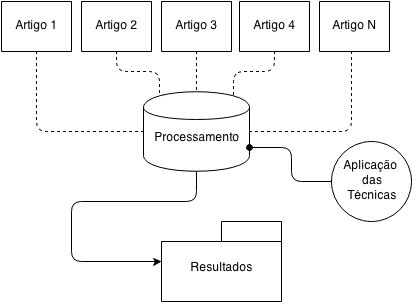
\includegraphics[width=0.7\linewidth]{./assets/introducao}
\end{figure}

\section{Contexto}

\comentario{Seção nova. Fala um pouco sobre de que maneira a ideia do trabalho surgiu. Peço que avaliem se este tópico não ficou muito pessoal. Tentei escrevê-lo o menos possível em primeira pessoa.}

\begin{textonovo}

A ideia desta pesquisa surgiu de uma necessidade pessoal durante a disciplina de Fundamentos da Ciência da Informação. Era necessária a leitura de um artigo científico de um determinado autor, porém, este era muito difícil de se encontrar disponível na Internet, o que fez com que tivesse de recorrer ao professor da disciplina para consegui-lo.

Após o envio deste artigo pelo professor, conforme solicitado, surgiu a seguinte reflexão:

\begin{quote}
\textit{''Esta contribuição ocorreu de maneira pessoal, entre mim e o professor, porém, se existisse um local onde os pesquisadores pudessem contribuir com o envio destes artigos este processo seria muito mais rápido e eficaz. Seria como se pudéssemos encontrar o artigo instantaneamente, dentro de nossa necessidade temporal. Seria pesquisador ajudando pesquisador.''}
\end{quote}

Desta forma, inclusive por minha formação acadêmica na área de Ciência da Computação, e por minha experiência profissional de mais de uma década em desenvolvimento Web, surgiu a ideia de desenvolver uma ferramenta de contribuição entre pesquisadores, totalmente online e independente. Todavia, estes repositórios de artigos já existiam na Internet e eram bem populados por sinal, porém, todos com um certo caráter comercial, com uma empresa ou instituição por trás, objetivando venda e lucro de uma maneira ou outra.

A ideia do desenvolvimento desta ferramenta ecoou durante dias, visto sua ampla aplicabilidade, como também sua contribuição social para com o universo da pesquisa, facilitando a vida de pesquisadores ao redor do mundo, sem complicações. Porém, para sua eficácia no armazenamento dos artigos enviados era necessária uma análise automatizada dos conteúdos destes arquivos, de maneira a extrair as partes mais importantes, como título, autores e referências, para que pudessem ser catalogados de maneira organizada e estruturada, a fim de facilitar a busca e permitir uma performance satisfatória por parte do usuário. Estes dados retirados dos documentos analisados são referenciados neste projeto pelo nome de ''metadados'', e são detalhados mais a frente de maneira aprofundada.

Sendo assim iniciou-se minha pesquisa pelo campo da extração de informação e principalmente pelo \textit{machine learning}, levando ao objeto central deste projeto, de maneira a identificar as características de cada ferramenta disponível atualmente e suas melhores aplicações dentro deste universo. Nada mais justo que contribuir com um projeto de pesquisa tendo como base fundamental o resultado de uma pesquisa acadêmica.

\end{textonovo}

\section{Problema}

\comentario{O problema foi reformulado, visando a identificação com o objetivo e resultados esperados.}

\begin{textonovo}
Diversas ferramentas e técnicas para extração de metadados em artigos podem ser facilmente encontradas com uma rápida pesquisa pela Internet. Porém, algumas são propriedade de universidades ou até mesmo de instituições privadas, o que dificulta sua análise e teste, visto que seu código fonte é fechado, ou seja, sem acesso.
\end{textonovo}

\begin{textoalterado}
As técnicas abordadas por este trabalho são aquelas cujo código fonte é aberto, ou seja, que pode ser analisado, testado e alterado, o que chamamos de projetos \textit{open source} (código livre).
\end{textoalterado}

De modo geral, estas técnicas livres de extração são focadas em \textit{layouts} (disposição visual) pré-definidos, geralmente seguindo modelos de conferências e/ou congressos internacionais, que possuem um padrão visual parecido, como é o caso do IEEE por exemplo, que serve de referência para diversos outros eventos da área da computação, tomando seu \textit{layout}, a princípio, como base.

Porém, existem diversos outros eventos que possuem \textit{layouts} de artigos considerados fora do padrão e, portanto, necessitam de adaptações destas técnicas para que seus trabalhos possam ser analisados e catalogados de maneira eficaz. Esta customização promoveria uma série de tentativas para verificar o melhor \textit{layout} para ser utilizado em cada caso, automaticamente.

\begin{textoalterado}
Algumas técnicas/ferramentas são aparentemente muito eficazes para um certo grupo de artigos, já seguindo um padrão visual pré-determinado. Porém, para alguns \textit{layouts} pouco comuns, de áreas do conhecimento diversas, espera-se que estas ferramentas não sejam tão eficazes, o que varia de acordo com a tecnologia aplicada e principalmente de acordo com o princípio teórico utilizado pelos seus autores, que será mais aprofundado nos próximos capítulos.
\end{textoalterado}

\section{Justificativa}

\comentario{Justificativa foi reformulada.}

\begin{textoalterado}
Interessante notar a necessidade de centralização de artigos científicos para o meio acadêmico, além de permitir à contribuição coletiva, que seria uma forma de aumentar cada vez mais o acesso aos materiais de pesquisa. 

Diante disso, esta extração de metadados automatizada e eficaz traria benefícios para que estes repositórios de artigos fossem criados e catalogados com precisão\end{textoalterado}, tendo então milhões e milhões de documentos em suas bases de dados, prontos para serem pesquisados por pesquisadores de todas as nacionalidades e áreas do conhecimento.

\begin{textoalterado}
Este trabalho busca, portanto, identificar a melhor maneira que isso pode ser feito, levando em consideração o melhor resultado matemático possível dentro das técnicas e ferramentes disponíveis atualmente. Este resultado traria, para tanto, um ganho científico incalculável, permitindo que novas ferramentas e repositórios fossem criados e a disseminação do conhecimento fosse cada vez maior, e mais rápida.
\end{textoalterado}

\section{Histórico}

\comentario{Nova seção. Resolvi colocá-la, porém de maneira breve, para que sirva de uma introdução sobre o assunto e principalmente demonstrar a ligação da Ciência da Informação com a Ciência da Computação.}

\begin{textonovo}

Os temas ''extração de informação'' e ''machine learning'' são resultantes da fusão de duas áreas do conhecimento bem complementares: a Ciência da Informação e a Ciência da Computação. Por esta proximidade, é muito comum encontrar artigos destes temas em ambas as áreas, porém com focos e objetivos diferentes.

Nesse sentido, essa união se complementa de maneira muito eficaz, visto a característica da fundamentação teórica da Ciência da Informação com a praticidade e desenvolvimento da Ciência da Computação. O resultado é um processo amplo e profundo, que permite que cada vez mais pesquisas sejam feitas e o ganho científico seja cada vez maior.

As pesquisas de \textit{machine learning} se iniciaram muito antes de se tornarem viáveis do ponto de vista tecnológico. Os primeiros registros desta pesquisa são datados de 1956 por \cite{machine-learning}, onde as primeiras teorias de aprendizado automatizado foram formuladas, utilizando-se para tal de conceitos matemáticos, defendendo a ideia do aprendizado por repetição e utilização de padrões.

Esta fundamentação ainda é muito utilizada e é a base para o desenvolvimento tecnológico existente na área de ''Inteligência Artificial''. Apesar de ser amplamente aplicada, os conceitos por trás desta fundamentação evoluíram ao longo das décadas, juntamente com a capacidade computacional, tornando os resultados muito mais reais e precisos do que era possível imaginar na formulação desta ideia.

Diante do cenário atual, com base no acelerado ritmo de desenvolvimento da tecnologia, bem como da evolução das técnicas de \textit{machine learning}, a utilização das ideias apresentadas décadas atrás ainda estão presentes e são amplamente utilizadas para o desenvolvimento de novas tecnologias e ferramentas.

Como é definido por \cite{foundations-machine-learning}, \textit{machine learning} atua como uma forma de aprendizado com base em experiências passadas, através da utilização de dados eletrônicos coletados que analisados posteriormente seguindo padrões definidos à máquina, de modo a permitir que ela possa fazer previsões com exatidão com base em sua experiência passada.

Este tema é muito amplo e sua aplicabilidade é extremamente ampla, permitindo a utilização de suas técnicas e teorias em diversas atividades, como classificação de textos e documentos, processamento de linguagem natural, reconhecimento de fala, detecção de fraudes, diagnósticos médicos e sistemas de recomendações, assim como mecanismos de buscas e extração de informação, ponto principal de discussão deste trabalho.

Dessa forma, este assunto tem sido discutido e pesquisado muito amplamente na Ciência da Informação, tanto nas áreas de classificação de documentos até mesmo em aplicações de buscas, unindo os conhecimentos adquiridos desta área do conhecimento com a evolução computacional presente nos dias atuais, onde a Ciência da Computação ganha força e nos permite realizar experimentos mais eficazes.

\end{textonovo}

\section{Objetivos}

\comentario{Os objetivos foram parcialmente reescritos, visando uma ligação maior com a metodologia, conforme observações feitas.}

\subsection{Objetivo Geral}

Este trabalho possui como objetivo geral \begin{textoalterado}identificar quais são as melhores técnicas de extração de metadados em artigos científicos e suas melhores aplicações, com base em um conjunto de documentos pré-selecionados para testes, dos mais diversos padrões e de diversas áreas do conhecimento.

Com efeito, esta identificação permite que resultados sejam comparados e confrontados, permitindo decidir qual técnica é melhor utilizada para cada padrão visual, abrangendo um conjunto cada vez maior de dados e tendo resultados cada vez mais precisos.

\end{textoalterado}

%A necessidade de adequação é uma tendência natural de qualquer ramo de atividade, de maneira a promover possibilidades de ferramentas auto-suficientes capazes de suprir as necessidades de grupos específicos de pesquisas, de eventos ou conferências, que possui padrões de apresentação de artigos personalizados e que demandam de uma análise diferenciada para que possa ser indexada e então analisada por sistemas de informação.

\subsection{Objetivos Específicos}

\begin{textoalterado}

Com base na diferenciação dos \textit{layouts} de artigos científicos, este trabalho tem como objetivos específicos identificar também pontos em que as técnicas de extração de metadados necessitam de adaptações por parte de seus usuários e desenvolvedores, permitindo desta forma uma ampliação do universo de aplicação e garantindo assim uma cobertura mais abrangente dos artigos científicos analisados.

Acredita-se que os padrões de extração existentes no mercado são, de maneira geral, insuficientes para suprir todos os padrões de artigos existente, limitando a apenas uma pequena parcela destes, dentro de um \textit{layout} específico, o que acaba gerando um desconforto e uma perda de credibilidade destas técnicas existentes atualmente.

\end{textoalterado}

\section{Resultados Esperados}

\comentario{Texto parcialmente alterado para prover uma maior identificação com o objetivo e o problema da pesquisa, de maneira a criar uma ligação entre eles.}

\begin{textoalterado}

As formas de extração de metadados em artigos científicos são geralmente baseadas em \textit{layouts}, ou seja, em pequenos pedaços onde certos dados devem ser extraídos. Porém em virtude da grande diversidade de materiais produzidos, dos mais diversos padrões visuais existentes, este \textit{layout} padrão - geralmente utilizado em artigos científicos - não se mostra eficiente na abrangência total das necessidades da comunidade científica mundial. 

\end{textoalterado}

Sobre este aspecto, espera-se que certos artigos científicos não tenham seus metadados analisados de maneira eficaz por todas as técnicas de extração analisadas, uma vez que \begin{textoalterado}adaptações no código seriam necessárias a fim de permitir que outros padrões visuais de artigos fossem também analisados, aplicando então um dos fundamentos do \textit{machine learning}, o aprendizado. 

\end{textoalterado}

\begin{textonovo}

Por fim, espera-se que, com esta análise aprofundada das técnicas existentes, as mais eficazes na extração de metadados sejam identificadas e analisadas, elevando então o ganho científico neste tema de suma importância para o desenvolvimento tecnológico.

\end{textonovo}

\section{Estrutura}

Esta pesquisa é estruturada iniciando com uma \begin{textoalterado} breve introdução sobre o tema; a apresentação do contexto da pesquisa, bem como sua origem e motivação; a definição do problema; a justificativa; o histórico do trabalho, demonstrando suas origens e fundamentos históricos; os objetivos gerais e específicos e, por fim, os resultados esperados.\end{textoalterado}

O segundo capítulo tem como base o referencial teórico feito através de uma RSL (Revisão Sistemática de Literatura), tendo como base \cite{Kitchenham}, que propõe um passo-a-passo para um revisão de literatura eficaz de modo a atingir os resultados desejáveis com a pesquisa.

No terceiro capítulo temos a metodologia para o desenvolvimento do trabalho, as técnicas que serão aplicadas e principalmente como serão feitas. \begin{textoalterado}Posteriormente, no capítulo quarto temos a análise e apresentação dos resultados, explicando como os testes foram realizados, os ambientes de teste criados e os resultados coletados.\end{textoalterado}

No quinto capítulo temos a discussão/conclusão, trabalhos futuros e considerações finais sobre o trabalho apresentado.


%\section{Limitações do Trabalho}
%
%Este trabalho limita-se aos artigos científicos difundidos na comunidade científica em formato PDF, excluindo aqueles em que seu conteúdo é disponibilizados através de imagens escaneadas de documentos físicos, o que impede, em um primeiro momento, de ter os textos analisados em sua forma original, sem necessidade de processamento extra a fim de obter todo o material textual contido em tais imagens. Além disso o trabalho pressupõe que a língua inglesa seja utilizada como padrão
%
%% Sobre os servidores com Windows
%
%Já na questão de testes de cada técnica de extração de metadados, as técnicas que serão selecionadas deverão ser de código livre/aberto, ou seja, ter seu uso liberado sem a necessidade de pagamento de licenças. Deste modo excluímos todas as técnicas que necessitam de \textit{softwares} proprietários para funcionar, por exigir licenças e fugirem das previsões de teste deste projeto. Assim, os projetos deverão necessariamente utilizar de linguagens de programação livres (ou de código aberto) e que rodem em sistemas operacionais derivados do Unix, como o Linux, por exemplo.



% Referencial Teórico
\chapter{Referencial Teórico}

% Falar sobre RSL

Visando obter uma revisão de literatura eficaz foi feita uma Revisão Sistemática de Literatura, com base no relatório técnico de \cite{Kitchenham}. Diante disso, o projeto se torna mais abrangente do ponto de vista de pesquisa literária e ao mesmo tempo mais restritivo, realmente realizando o estudo dos objetos que são importantes para a pesquisa e seus resultados.

% Bases pesquisadas

Como o objetivo do trabalho tem foco na resultado prático, geralmente as bases relacionadas às áreas mais técnicas, como Ciência da Computação, devem ser bem focadas, como IEEE e ACM, por exemplo. Outras bases de natureza mais genérica também foram pesquisadas, geralmente através do site da CAPES, mas com caráter mais de apoio teórico realmente.

Embora a amplitude desta área de estudo, alguns detalhes necessitam ser observados para evitar assim redundância e perda de foco. A pesquisa necessitava ser focada em técnicas de extração de metadados em artigos científicos, somente. Estas técnicas necessitam ser reais, de maneira a existir realmente uma forma prática de serem testadas, fazendo assim com que os resultados obtidos sejam comparados e confrontados para verificar então a eficácia deste processo.

Como a pesquisa necessita de um resultado prático eficaz os critérios que serão adotados para demonstrar a relevância de um estudo serão seus resultados. Com base em uma técnica potencialmente eficaz, esta deve ser testada juntamente com um grupo de artigos previamente selecionados. Estes artigos já possuirão seus dados mapeados de maneira a poder comparar os resultados obtidos com cada uma das técnicas e seus respectivos resultados. Portanto os critérios utilizados serão de natureza explicitamente prática, com foco em resultados concretos, numericamente representados.

% Falar sobre os eventos encontrados na área

Seguindo as orientações propostas em \cite{Kitchenham} foram mapeados alguns eventos para serem pesquisados, a fim de encontrar trabalhos relevantes para a área. Sendo assim, foram mapeados os seguintes eventos:

\begin{itemize}
\item KDIR (International Conference of Knowledge Discovery and Information Retrieval)
\item ICDAR (International Conference on Document Analysis and Recognition)
\item PDCAT (International Conference on Parallel and Distributed Computing, Applications and Technologies)
\item IAPR (International Workshop on Document Analysis Systems)
\item ACM Conference on Digital Libraries
\end{itemize}

\begin{textoalterado}
Estes eventos foram analisados, observando todas as citações e referências utilizadas, a fim de encontrar também detalhes importantes para a pesquisa, sem perder o foco do trabalho.
\end{textoalterado}

\section{Metadados}

\comentario{Esta nova seção foi incluída para definir alguns conceitos que são apresentados mais a frente com a apresentação das técnicas.}

\subsection{Conceito de Metadado}

\begin{textonovo}

Com base nas ideias apresentadas por \cite{meta-dados}, podemos definir inicialmente um metadado da seguinte maneira:

\begin{quote}
\textit{''[...] an element of metadata describes an information resource, or helps provide access to an information resource.''}
\end{quote}

Sobre este aspecto conclui-se que todo dado que agregue nova informação a um recurso pode ser considerado um metadado. Desta maneira, quanto mais metadados um recurso tiver, mais detalhado ele é, ou seja, mais dados sobre ele temos. Com efeito, podemos simplificar ainda mais a definição de metadado com sendo \textit{um conjunto de dados sobre um determinado recurso}.

Temos contato diariamente com diversos metadados, sejam eles visíveis naturalmente ou não, mas de uma maneira ou outra, são utilizados em tarefas do cotidiano de maneira ampla; geralmente um conjunto enorme de novos dados e informações sobre recursos dos mais diversos tipos e modelos.

Podemos citar, por exemplo, a utilização de pequenos pedaços de dados sobre um conjunto de livros, dentro de um ambiente de biblioteca, por exemplo, o que é considerado uma coleção de elementos de metadados, conforme pode ser confirmado em \cite{meta-dados}. Além disso, o mesmo autor cita como exemplos de metadados os dados coletados por mecanismos de busca no momento em que as páginas da Internet são indexadas e então armazenadas.

Ante o exposto, podemos criar e identificar diversos conceitos do que podemos chamar de metadado, porém, em virtude de sua enorme aplicação e significância, alguns detalhes dentro do escopo deste trabalho devem ser direcionados, visando identificar e explicar melhor os conceitos que serão aplicados na análise das ferramentas e técnicas que aqui serão apresentadas.

\end{textonovo}

\subsection{Padrões de Metadados}
\label{padroes-de-metadados}

\begin{textonovo}

Diante da infinidade de dados que podem estar atrelados a um recurso, temos uma amplitude muito grande de características que podem ser definidas como sendo metadado. Por isso, foram definidos 15 (quinze) elementos de metadados para descreverem um recurso informacional, independente da disciplina em questão, estabelecendo então um padrão. 

Para isso, foi criado o padrão Dublin Core \cite{dublin-core}, que se originou após uma série de encontros feitos desde 1995, unindo bibliotecários e pesquisadores digitais e de conteúdo, visando identificar padrões para se representar um recurso eletrônico, seja ele uma página, um texto ou até mesmo um documento em um determinado formato. O nome ''Dublin'' foi dado em virtude da primeira reunião do grupo, que foi realizada em Dublin, Ohio. Já o nome ''core'' se deu em virtude dos elementos serem amplos e genéricos, sendo então utilizados para descrever uma grande variedade de recursos.

Os quinze elementos que fazem parte do padrão Dublin Core compartilham de um vasto conjunto de vocabulários de metadados, juntamente com diversas especificações técnicas, que são mantidas pela Dublin Core Metadata Initiative (DCMI), a agência responsável pela definição destes elementos.

Este padrão é utilizado nos dias atuais para se representar um recurso na Internet, por exemplo, podendo ser qualquer coisa que possa ser identificada \cite{dublin-core-1-1}. Com base em suas características, mecanismos de busca podem indexar um recurso de maneira mais rápida e precisa, pois este é acompanhado de pequenas sinalizações sobre seu conteúdo, que são os metadados. 

Para cada elemento descrito pelo padrão temos informações como: 

\begin{itemize}
\item \textit{label}, que é o texto para leitura e entendimento humano;
\item \textit{name}, que é usado para o processamento de máquina, ou seja, um identificador que a máquina utiliza para reconhecimento.
\end{itemize}

Os elementos que fazem parte da versão 1.1 do padrão Dublin Core \cite{dublin-core-1-1} podem ser vistos no \refanexo{anexo-dublin-core} deste trabalho.

Abaixo podemos ver um exemplo de código para utilização de metadados Dublin Core em uma página da Internet, por exemplo, onde iremos referenciar os elementos \textit{creator}, \textit{title} e \textit{language}.

\lstset{language=HTML}
\begin{lstlisting}[escapechar=\#]
<meta name="DC.Creator" content="Junior Grossi" >
<meta name="DC.Title" content="#\imprimirtitulo#" >
<meta name="DC.Language" content="pt_BR" >
\end{lstlisting}

Desta forma, a indexação do autor (\textit{DC.Creator}) da página, bem como seu título (\textit{DC.Title}) e idioma (\textit{DC.Language}), são feitos de maneira bem simplificada e direta. Para páginas da Internet, com as informações todas em formato HTML, a utilização destes metadados perderiam o sentido, visto que essas informações poderiam ser facilmente encontradas de outras formas, como a análise do próprio código HTML. Porém, para documentos binários - em formato PDF ou Word, por exemplo - a utilização destes metadados é de suma importância, visto que permite que essas informações básicas sejam capturadas sem a necessidade de análise do conteúdo dos arquivos, o que traria complexidade ao processo.

\end{textonovo}

\subsection{Técnicas de Extração de Metadados}

Algumas técnicas e algoritmos de extração de metadados são utilizadas em diversos projetos, de maneira a serem citadas em momentos onde exige-se uma precisão maior.

Estas técnicas se baseiam basicamente na classificação de dados com base nas suas representações escritas, tanto baseadas em padrões preestabelecidos ou até mesmo com base em um dicionário de palavras capaz de reconhecer ocorrências em diversas partes de um documento, o que agrega assertividade ao processo de extração.

\subsubsection{Support Vector Machines (SVM)}

\begin{textonovo}
Support Vector Machines (SVM) é uma técnica de \textit{machine learning} que permite que um conjunto de dados sejam analisados, possibilitando que padrões sejam extraídos, criando uma espécie de memória, através de classificação.

Esta técnica se baseia na redução de erros com base em um resultado de treinos consecutivos que permitem a criação de um padrão e estabelecem um aprendizado por parte do reconhecimento de padrões \cite{vapnik-svm}. Todas as análises realizadas são mapeadas, permitindo que um registro histórico em forma matemática seja realizado, levando o algoritmo à possibilidade de diferenciação entre um resultado e outro, de forma numérica.
\end{textonovo}

\begin{textoalterado}
Vários algoritmos de extração se baseiam na utilização de SVM como técnica principal, visto sua eficiência no reconhecimento de padrões. Como descrito por \cite{svm} a utilização desta técnica é baseada na identificação de campos previamente selecionados no cabeçalho de um documento, do qual se deseja obter os metadados.

Esta técnica analisa diversos campos chamando-os de classes, e atribui a cada classe uma característica que a permite ser identificada. Deste modo, cada linha do cabeçalho do documento é classificada em uma ou mais classes, que fazem parte do padrão Dublin Core, detalhado na \autoref{padroes-de-metadados}.
\end{textoalterado}

\begin{textonovo}
Estes campos são mapeados em uma representação bidimensional, permitindo identificar visualmente os padrões encontrados na análise de cada classe. Desta forma, com a visualização do posicionamento de cada ocorrência é possível obter uma distância clara entre os pontos de reconhecimento, chamada pelo autor de \textit{hyperplanes} \cite{vapnik-svm}. Por sua vez, estes pontos são marcados como sendo os ''support vectors'', que permitem que o \textit{hyperplane} entre eles determine a divisão entre as classes de forma clara e eficaz, como pode ser visto na \autoref{fig:svm-grafico}. Esta divisão então permite a distinção entre os metadados, diferenciando então os elementos analisados pelo algoritmo.
\end{textonovo}

\begin{figure}
	\centering
	\caption{Distância representando a separação entre classes na técnica de SVM.}
	\label{fig:svm-grafico}
	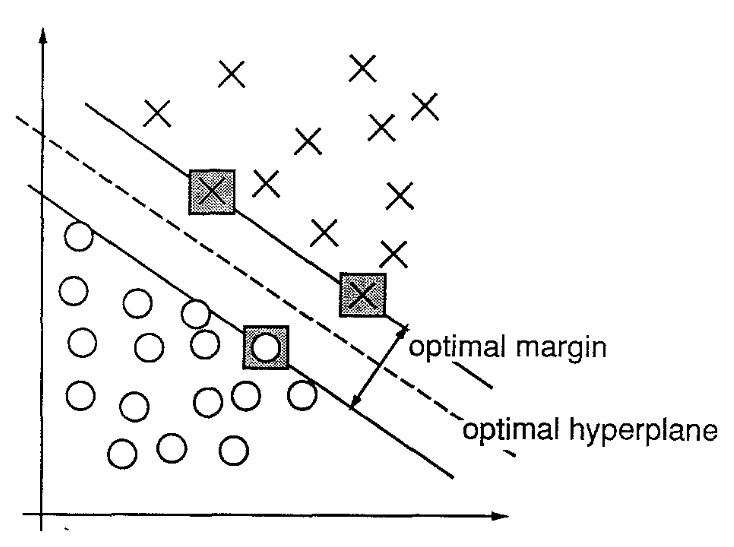
\includegraphics[width=0.6\linewidth]{./assets/svm-grafico}
\end{figure}


% % % % % % % % % % % % % % % % % % % % % % % % % % % % % % % % % %
% % % % % % % % % % % % % % % % % % % % % % % % % % % % % % % % % %
% Falar mais de SVM, suas aplicações além da IE e inclusive da IE %
% % % % % % % % % % % % % % % % % % % % % % % % % % % % % % % % % %
% % % % % % % % % % % % % % % % % % % % % % % % % % % % % % % % % %












\section{Revisão de Estado da Arte na Extração de Metadados}

\section{Técnicas de Algoritmos}

\section{Ambientes de Extração de Metadados}

% % % % % % % % % %

\section{Técnicas e Algoritmos}





\begin{table}
    \caption{Relação de classes utilizadas e comparação com o padrão Dublin Core.}
    \begin{center}
        \begin{tabular}{|C{3cm}|C{3cm}|p{7cm}|}
            \hline \textbf{Classe (Tag)} & \textbf{Referência Dublin Core} & \textbf{Descrição}\\ 
            \hline Title & Title & Título do artigo\\
            \hline Author & Creator & Nome do autor do documento\\
            \hline Affiliation & & Afiliação do autor\\
            \hline Address & & Endereço do autor\\
            \hline Note & & Frases de reconhecimentos, \textit{copyright}\\
            \hline Email & & Endereço de e-mail do autor\\
            \hline Date & & Data da publicação\\
            \hline Abstract Introdution & Description & A parte de introdução do artigo\\
            \hline Phone & & Telefone do autor\\
            \hline Keyword & Subject & As palavras-chave do documento\\
            \hline Web & & Endereço na Internet do autor\\
            \hline Degree & & Associação com o grau acadêmico\\
            \hline Pubnum & & Número da publicação do documento\\
            \hline Page & & O final da página\\
            \hline
        \end{tabular}
    \end{center}
    \label{tab:svm-classes}
\end{table}

Para o caso de extração de metadados em artigos científicos utilizando \textit{Support Vector Machines} \cite{svm} as tags de Seymore et al. \cite{seymore} são utilizadas para representação destas classes.

Deste modo, com base nestas classes são definidas características de suas classes vizinhas, como por exemplo, elementos que ficam perto de outros elementos, que possuem uma sequência lógica geral de exibição. Com base nestas informações, que são feita classe por classe, estes padrões vão sendo encaixados a cada linha do cabeçalho analisado, permitindo que os metadados sejam extraídos com uma grande precisão.

Além da análise linha por linha são utilizadas análises de palavras dentro de um contexto previamente selecionado. Assim foi criado um \textit{cluster} de palavras comuns que facilitam na identificação destas classes nos cabeçalhos analisados. Este \textit{cluster} basicamente é composto de:

\begin{itemize}
\item Dicionário online padrão em sistemas Linux;
\item 8441 nomes e 19613 sobrenomes;
\item Sobrenomes chineses;
\item Nome dos estados do Estados Unidos e das províncias canadenses;
\item Nomes das cidades dos Estados Unidos;
\item Nome dos países do mundo, de acordo com World Fact Book\footnote{Disponível em \url{https://www.cia.gov/library/publications/the-world-factbook/index.html}};
\item Nome dos meses e suas respectivas abreviações.
\end{itemize}

Para cada uma das classes analisadas são feitas correlações com o tipo de dado esperado, de maneira a permitir que endereços de e-mail, por exemplo, sejam extraídos com base em expressões regulares utilizadas em linguagens de programação.

\subsection{Hidden Markov Models (HMM)}

A teoria básica de Markov foi conhecida próximo dos anos 80 por engenheiros e matemáticos com grande aplicação inicialmente em processamento da fala mas com vasta amplitude em outras áreas onde descoberta de padrões pode ser aplicada \cite{hmm}.

O processo é baseado na identificação de modelos observáveis que representem e caracterizem a ocorrências de símbolos observáveis, ou seja, padrões. Se um sinal foi observado ele pode ser utilizado para futuras referências, de acordo com o padrão observado.

Um exemplo prático citado por Rabiner e Juang \cite{hmm} é o caso de uso do jogo  \textit{Cara e Coroa}. Toma-se um observador em um quarto fechado com uma cortina totalmente fechada para outro cômodo. Este observador não consegue ver nada que acontece no outro cômodo, onde está uma outra pessoa jogando uma moeda pra cima, relatando sempre o resultado obtido (cara ou coroa). Neste caso o problema é construir um Hidden Markov Model (HMM) para explicar ao observador a sequência dos resultados obtidos. 

Este exemplo é baseado tanto no estado de cada resultado (cara ou coroa) e em probabilidades matemáticas de ocorrência destes estados, neste caso 50\%. Assim desenha-se modelos onde os estados são representados com base nas inúmeras possibilidades existentes, levando inclusive em consideração a sequência dos fatos, ou estados.

No âmbito da extração da informação, o HMM pode ser aplicado conforme é apresentado por Seymore et al. \cite{seymore}, onde um modelo construído manualmente contendo múltiplos estados por campos (título, autor, etc), pode ser mais eficiente do que um modelo com um estado por campo. 

%Seymore et al. \cite{seymore} definiu também 15 (quinze) tags para esta definição do cabeçalho de um documento. Porém, destas 15 (quinze) tags definidas, somente 4 (quatro) correspondem ao padrão da Dublin Core e estão ilustradas na \autoref{tab:svm-classes}.

\begin{figure}
\centering
\caption{Exemplo de modelo HMM, onde X são os estados, Y as observações possíveis, A as probabilidades de mudança de estado e B as saídas das probabilidades.}
\label{fig:hmm-states}
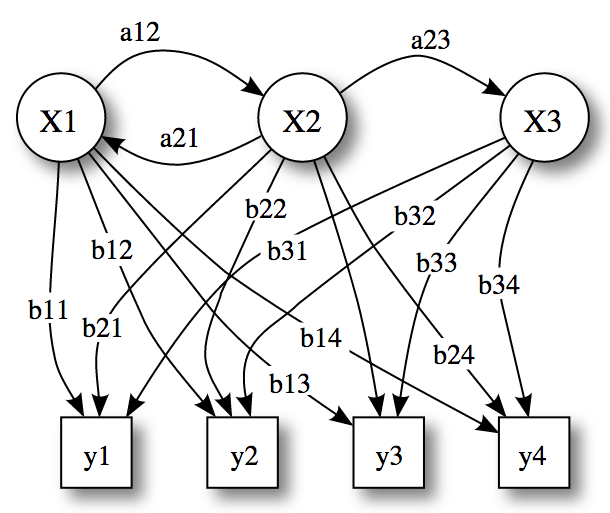
\includegraphics[width=0.7\linewidth]{./assets/hmm-states}
\end{figure}

Um dos pontos positivos deste modelo é que por serem baseados em estatística eles são muito bem empregados em domínios de linguagem natural, aliando os resultados positivos à excelente performance computacional. Como desvantagem deste método podemos citar o fato de, por ser baseado em estatística, uma grande quantidade de dados deve ser utilizada a título de treino para obter os número significativos para então ser aplicados de maneira final.

Deste modo, para extração dos metadados o HMM pode ser utilizado aplicando um marcador (\textit{label}) em cada palavras do cabeçalho de um documento (artigo científico), relacionando cada uma a uma classe, como título, autor, etc.

\subsection{Word Clustering}

Utilizando de trabalhos tradicionais, como \cite{svm}, Han et al. \cite{rule-based} apresentou uma ideia de um \textit{cluster} de palavras para promover a extração de metadados de documentos, indo de maneira relativamente contrária às propostas tradicionais, baseando apenas na ocorrência e estatísticas de palavras isoladas.

Técnicas baseada em \textit{cluster} de palavras geralmente apresentam performance maiores do que as técnicas tradicionais \cite{rule-based}. Este grupo de palavras demonstra relação entre palavras semelhantes dentro de um contexto, permitindo que a extração dos metadados possa ocorrer de maneira mais eficaz.

Han et al. agrupou bases de dados de domínios diversos incluindo também propriedades ortográficas de palavras, que possuem conhecimento prévio de classes específicas, como autor, título, etc. Deste modo palavras encontradas nos documentos vão sendo comparadas com palavras deste \textit{cluster}, permitindo identificar por grupos características de metadados, como por exemplo, a palavra ''Mary'' faz parte do contexto de ''nomes'', portanto existe uma probabilidade maior de ela, juntamente com seu grupo de palavras ao redor fazerem parte da classe ''autor'' por exemplo. Esta lógica é apresentada para outras classes, como ''e-mail'' por exemplo, que pode ser identificado, em sua grande maioria, com a presença do caractere ''@''.

\begin{figure}
\centering
\caption{Workflow da extração de metadados usando \textit{cluster} de palavras}
\label{fig:workflow-rule-based}
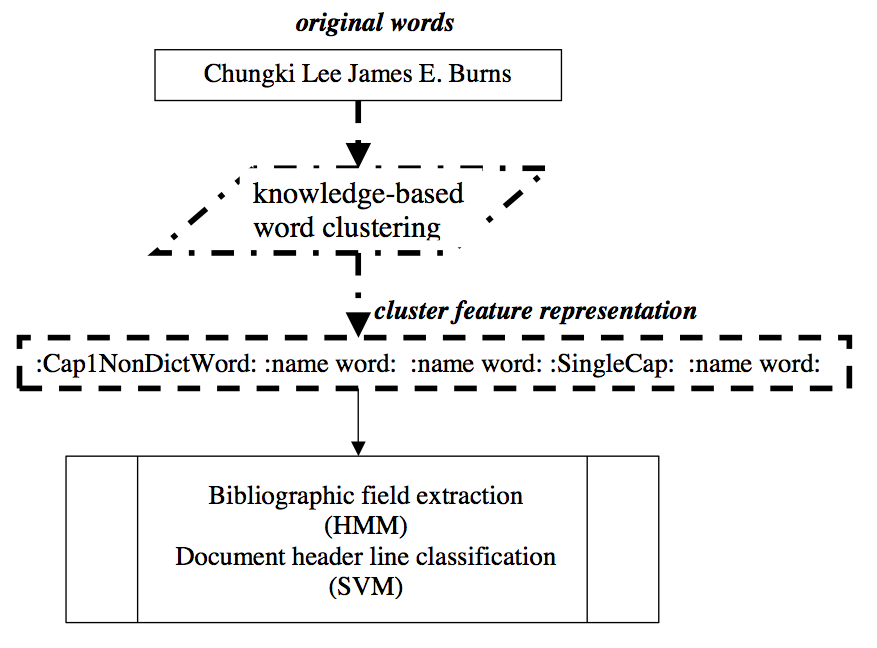
\includegraphics[width=0.7\linewidth]{./assets/workflow-rule-based}
\end{figure}

Han et al. ainda utiliza da técnica  de SVM (Support Vector Machines) para classificação de linhas de um cabeçalho de um documento, tanto em função dos bons resultados obtidos quanto também pela boa performance apresentada. Deste modo, cada linha obtida se transforma em um vetor de palavras, que é comparado com o \textit{cluster}, identificando mais facilmente os metadados.

Além disso é utilizada também a técnica de HMM \cite{hmm2} para a extração das referências, observando sempre a ocorrência de padrões como título e autor para identificação dos mesmos em referências existentes no documento.

Basicamente a \textit{Rule-based Word Clustering} se resume em 3 (três) etapas. A primeira etapa se resume na construção das bases de dados, assim como \cite{svm}, onde foram utilizadas também como bases externas os nomes apresentados em seu \textit{cluster} de maneira a unir não somente estas bases externas mas também bases construídas dentro de um domínio específico, como palavras que fazem parte de um conjunto finito, não genérico.

A segunda etapa é chamada de \textit{Cluster Design}. Esta etapa é onde os \textit{clusters} são arquitetados, de maneira a contemplar também propriedades ortográficas das palavras, como se funcionasse de maneira geral como uma expressão regular de palavras, formando então um \textit{cluster} com base nas características apresentadas.

A terceira etapa é chamada de \textit{Rule Design}, que resume-se basicamente na representação de cada palavras dentro de seu contexto de apresentação. Por exemplo, nomes devem começar com a primeira letra maiúscula para então serem classificadas como do grupo de ''nomes''.

Como resultado este \textit{cluster} permite um ganho considerável de performance, além de permitir uma precisão maior dos resultados, visto que eles são apresentados com base nestas bases focadas em um domínio específico, perfazendo um contexto mais definido e com resultados mais garantidos ao se comparar por exemplo com técnicas de \textit{cluster} distribuídos.

Por outro lado a utilização desta técnica possui uma falha em semântica dos dados, visto que quando um dígito ou conjunto deles é substituído por \texttt{:number} ele se torna apenas um número, sem um contexto específico, ou seja, pode ser tanto uma referência a alguma página ou até mesmo um mês de um ano.

\subsection{Conditional Random Fields (CRFs)}

% Falar sobre CRFs 

Conditional Random Fields é um framework proposto por Lafferty et al. \cite{crf} criado para construir modelos probabilísticos e dados marcados em sequência (\textit{label sequence data}), geralmente utilizados no reconhecimento de padrões e aprendizado de máquinas (\textit{machine learning}).

Sua representação é puramente matemática com modelos gráficos a fim de maximizar as probabilidades condicionais que se desejam aplicar.

Esta técnica é comparada e quase sempre utilizada juntamente com a HMM (Hidden Markov Models), de maneira a possuir algumas vantagens sobre esta última, como a habilidade de relacionar pressupostos independentes nos modelos, ou seja, relacionar observações e/ou interpretações.

Além disso, CRFs são utilizadas também em marcação e parseamento de dados sequenciais, com uma ordem determinada, como linguagem natural, sequências biológicas (como os genes) ou estados computacionais.

% Falar sobre o uso de CRFs na extração de informação

Sua aplicação na extração de metadados foi apresentada por Peng et al. \cite{crf-ie}, como uma maneira eficaz de extrair padrões em cabeçalhos e referências de artigos científicos. Deste modo, através da identificação destes padrões sequenciais pode-se determinar os tipos de dados existentes e então identificá-los, seguindo uma lógica/ordem pré-determinada.

A utilização de CRFs na extração de metadados mostra-se muito eficaz por reduzir bastante os erros em algumas métricas, aumentando o sucesso da aplicação desta técnica nesta área.

\section{Trabalhos Comparativos}

\comentario{Falar sobre as comparações realizadas por Granitzer, tanto no que diz respeito a layouts \cite{granitzer-layout-based}, quanto no que diz respeito a dicionários \cite{Granitzer2011a}.}

\section{Ferramentas e Projetos de Destaque}

Alguns projetos baseiam sua extração em padrões pré-definidos de maneira a identificar dados relevantes dentro de uma região específica, facilitando a procura e consequentemente aumentando a velocidade no resultado. 

Estes projetos geralmente permitem uma variedade muito grande de layouts, embora nem todos já estejam previamente definidos. Geralmente novos layouts são inseridos em novas versões ou até mesmo por contribuições das mais diversas, como é o caso dos projetos de código livre, os chamados projetos \textit{open source}.

Abaixo segue uma relação dos principais projetos relacionados à área de extração de metadados de artigos científicos, com informações sobre seu funcionamento e algoritmos que são utilizados.

\subsection{Cermine}

% CERMINE

Um destes projetos é o recente CERMINE \cite{cermine}, uma biblioteca \textit{open source} desenvolvida na linguagem de programação Java que permite que sejam extraídos os metadados de artigos científicos em formato digital PDF, oferecendo ainda a possibilidade de cruzamento de dados por meio de referências e títulos, permitindo assim identificar citações bem como a relevância de um determinado documento.

O CERMINE ainda possui um mecanismo de aprendizagem da própria máquina, permitindo que na medida que dados forem sendo alterados ele consiga absorver os detalhes e permitir assim uma mudança de sua maneira de extrair os dados. Deste modo ele permite que seja adaptado para novos padrões de layouts, o que permite de maneira geral que uma grande gama de modelos seja então abrangida. 

Seu grande diferencial em comparação com as demais técnicas é que ele não somente extrai os metadados de um artigo, mas sim analisa todo o seu conteúdo, incluindo citações a outros artigos, que podem ser facilmente cruzados por meio de informações como título e autor(es).

Seu mecanismo considera somente arquivos PDF com texto gerado de maneira pura, sem a utilização de imagens. Basicamente ele considera regiões, linhas e páginas como pontos estratégicos para a extração de informações. As bases destas regiões possuem padrões que são utilizados juntamente com técnicas de SVM \cite{svm}. Com base nisso ele condensa um layout onde as informações geralmente estão dispostas, permitindo assim que em um determinado local do arquivo esteja, provavelmente, o título e o nome dos autores. 

Com estas regiões definidas o CERMINE extrai as informações com base em padrões preestabelecidos, de maneira a gerar então sua saída para os metadados e sua saída para as referências encontradas. A saída trabalhada pelo projeto é no formato XML, permitindo assim que possa ser compartilhado com outros sistemas por possuir uma leitura semântica e ao mesmo tempo fácil de ser interpretada pelas linguagens de máquinas. A \autoref{fig:cermine-workflow} demonstra como o processo de extração do CERMINE funciona.

\begin{figure}
\centering
\caption{CERMINE Extraction Workflow}
\label{fig:cermine-workflow}
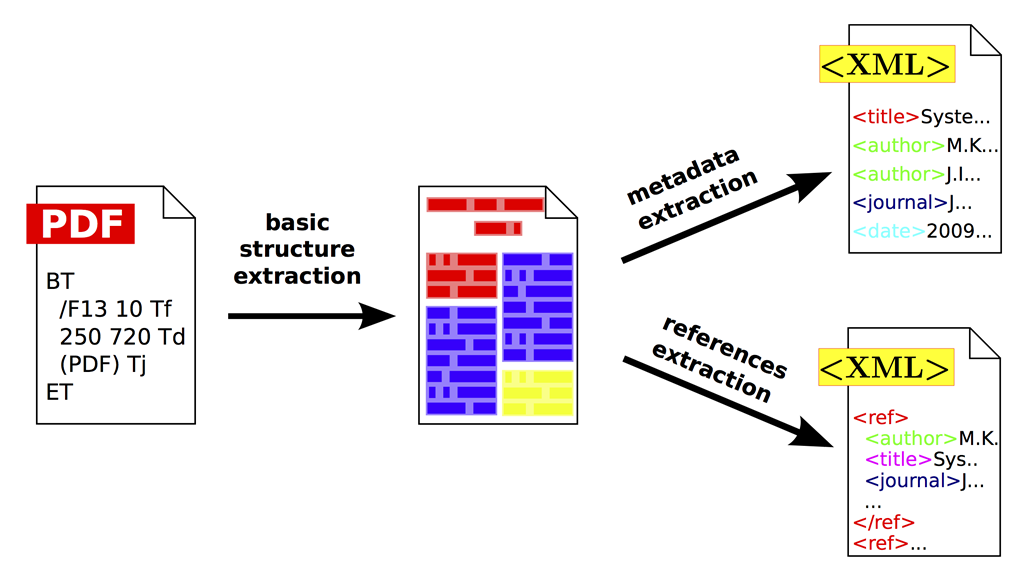
\includegraphics[width=0.7\linewidth]{./assets/cermine}
\end{figure}

Com o mapeamento definido ele identifica regiões de acordo com seu conteúdo, as quais ele chama de \textit{zones}. Esta regiões são determinadas a fim de extrair as informações relevantes para cada uma, de maneira a separar, por exemplo, a área destina aos metadados do arquivo. O CERMINE divide estas \textit{zones} da seguinte maneira:

\begin{itemize}
\item \textbf{Metadata:} É a região mais ao alto do documento, onde obtém os metadados, que seriam o resumo, \textit{bib\_info}, tipo, título, afiliação, autores, datas, editores e palavras-chaves.
\item \textbf{References:} Região responsável por identificas detalhes de referências que foram utilizadas no artigo, como título e autores, por exemplo
\item \textbf{Body:} O texto geral do artigo, incluindo equações, imagens e tabelas.
\item \textbf{Other:} Outros detalhes menos significantes semanticamente, como número das páginas, dentro outros.
\end{itemize}

A extração das referências abrange também seus próprios metadados. Tanto no texto corrido (\textit{Body}) quanto na lista de referências do artigo o \textit{parser} do CERMINE analisa linha a linha, permitindo uma extração de dados mais eficaz. Das referências são extraídos os seguintes dados: autor, título, nome do \textit{journal}, volume, \textit{issue}, páginas, \textit{publisher}, localização e o ano.

\subsection{TeamBeam}

Outros projeto de destaque é o TeamBeam \cite{teambeam}, cuja base ideológica possui objetivos bem sociais, de contribuir com o compartilhamento de conhecimento. Basicamente o objetivo do projeto é extrair metadados de artigos científicos, porém focado apenas nestes, de maneira a extrair título, nome do \textit{journal}, resumo e informações sobre os autores, como nome, endereço de e-mail e afiliações.

O projeto também é de código livre (\textit{open source}) e é baseado na extração de pequenos blocos de texto. A manipulação dos arquivos PDF são feitas pela biblioteca PDFBox \footnote{Biblioteca de manipulação de arquivos PDF mantida pela Fundação Apache. Disponível em \url{https://pdfbox.apache.org/}}, que fornece meios eficazes de extrair textos com base nas regiões desejadas.

O algoritmo do TeamBeam utiliza o algoritmo de \textit{Maximum Entropy} \cite{maximum-entropy}, que utiliza basicamente de tarefas de classificação sequencial como ferramenta principal para obtenção de padrões. A base deste algoritmo está na utilização de CRFs \cite{crf}, principalmente no que diz respeito à extração dos metadados \cite{crf-ie}.

O processo de extração é feito basicamente em duas etapas. A primeira é a etapa de classificação de blocos de texto (\textit{text block classification}), onde geralmente já é possível obter algum dado concreto de resultado. Neste etapa o objetivo é associar certos blocos de texto a um dos seguintes marcadores: \textit{Title Block}; \textit{Sub-Title Block}; \textit{Journal Block}; \textit{Abstract Block}; \textit{Author Block}; \textit{E-Mail Block}; \textit{Affiliation Block}; \textit{Author-Mixed Block}; e \textit{Other Block}.

Dependendo do layout do artigo alguns metadados podem vir divididos em blocos de texto diferentes, necessitando de um processamento posterior, como é o caso, geralmente, dos blocos com informações sobre os autores. Neste caso também é realizada a etapa de classificação de token (\textit{token classification}), que se resume na classificação de palavras individualmente de acordo com um dos seguintes marcadores: \textit{Given Name}; \textit{Middle Name}; \textit{Surname}; \textit{Index}; \textit{Separator}; \textit{E-Mail}; \textit{Affiliation-Start}; \textit{Affiliation}; e \textit{Other}.

Kern et al. defendem a ideia dos excelentes resultados do TeamBeam ao ser comparado com outros projetos. Este fato é dado em virtude das características que são levadas em consideração no processamento do algoritmo, utilizando de dicionários, informações de layout e modelo de linguagem.

\subsubsection{Resultados Comparativos}

A fim de analisar os resultados obtidos com a aplicação das técnicas descritas no TeamBeam, os autores comparam as técnicas utilizadas com outras técnicas de outras ferramentas, que utilizam processos diferentes de análises.

Para fins de comparação de resultados, os autores citam as técnicas ParsCit (\autoref{tec-parscit}), Layout-CRFs (\autoref{tec-layout-crfs}) e Mendeley Desktop (\autoref{tec-mendeley}). Como conclusão ele compara estas três técnicas separadamente, por não abrangerem todos os detalhes que o TeamBeam possui, o que tornaria a comparação desleal.

Assim, ele chega à conclusão que em virtude das diferentes formas de processamento dos dados feitas por cada umas das ferramentas, chega-se a resultados mais precisos para cada campo extraído. Por exemplo, o Layout-CRF's (\autoref{tec-layout-crfs}) é mais abrangente e mais assertivo para extração de títulos, por ser baseado em CRF. Já as ferramentas baseadas em dicionário apresentam melhores resultados para extração de autores, visto se basearem em \textit{data-sets\footnote{Bases de dados com nomes dos autores mais citados e outras informações já catalogadas que são armazenadas para consulta pública.}} já consolidados.

\comentario{Devo explicar aqui o que seriam esses Data-Sets? Exemplo: E-Prints, Mendeley e PubMed.}

\subsection{Layout-CRF's}
\label{tec-layout-crfs}

\comentario{Escrever sobre.}

\subsection{Mendeley Desktop}
\label{tec-mendeley}

\comentario{Escrever sobre.}

\subsection{CiteULike}
\label{tec-citeulike}

\comentario{Escrever sobre CiteULike, com base no artigo de seus autores \cite{citeulike}.}

\subsection{CiteSeer}

Um dos projetos mais específicos encontrados é o CiteSeer \cite{citeseer}. Seu objetivo não é apenas extrair dados em artigos, mas sim também analisar citações de outros documentos no conteúdo textual encontrado. Assim, ele é capaz de identificar quais documentos são citados, quantas vezes são citados e onde são citados, se assemelhando muito ao processo de citação natural.

Desta forma, com estas informações identificadas, ele consegue criar um \textit{ranking} dos documentos citados, incluindo seus autores e \textit{journals}, criando a partir de um documento fonte todo um conjunto de relações com outros documentos de uma maneira estatística bem eficaz.

Os indexes de citações (\textit{citation indexes}), que são utilizados no projeto, foram originalmente criados para a recuperação de informação, porém sua utilidade é tamanha que permite que citações sejam indexadas de maneira eficaz, permitindo inclusive que referências de documentos em idiomas diferentes sejam identificadas. Desta maneira, essa técnica pode ser utilizadas de diversas formas, não somente na identificação de citações propriamente ditas, mas envolvendo um conjunto de informações eficazes, como inclusive identificar a reputação de um determinado artigo científico no meio em que se encontra, simplesmente analisando onde é referência em relação ao número de vezes em que é citado.

Uma proposta interessante em que se baseia o CiteSeer é a de Cameron \cite{cameron}. Seu objetivo é de formar uma Base de Citações Universal, onde todos os artigos estariam ligados entre si, independente de qualquer fator externo como idioma, por exemplo. A diferença entre esta proposta e o trabalho realizado com o CiteSeer é que este último permite que os documentos sejam analisados sem nenhum esforço extra, ou seja, sem a intervenção dos autores dos documentos, como é proposto por Cameron. Neste caso, os documentos seriam analisados de maneira automática, diminuindo o tempo necessário para o relacionamento de todos eles e aumentando a eficácia e eficiência do processo.

O funcionamento do CiteSeer é relativamente simples, porém o trabalho realizado por detrás do processo envolve muito estudo e dedicação. Basicamente ele é capaz de fazer o \textit{download} de \textit{papers} utilizando a Internet, convertê-los em texto e realizar a análise de todas as suas citações. Este resultado é armazenado em um banco de dados para consultas e relacionamentos futuros. Um dos pontos interessantes desta análise é que como ela é feita com base em referência textual, identificado origem e destino, ela pode ser facilmente aplicada tanto no sentido natural de leitura (um artigo cita outros) quanto no sentido inverso (um artigo é citado por outros). 

O projeto também possui suas desvantagens, como por exemplo, a não cobertura de alguns \textit{journals} importantes, indexando todos seus documentos online e de maneira automática. Além disso o projeto original não é capaz de identificar mais de um autor nos documentos, sendo a identificação apenas pelo campo autor, tendo ele apenas um ou mais de um pesquisador envolvido.

Basicamente o projeto analisa o documento em partes:

\begin{itemize}
\item \textbf{URL:} a URL onde o documento foi obtido;
\item \textbf{Cabeçalho:} o bloco de título e autor do documento;
\item \textbf{Resumo:} o bloco de resumo do documento;
\item \textbf{Introdução:} a introdução do texto do documento;
\item \textbf{Citações:} a lista de referências a outros documentos citadas no decorrer do texto;
\item \textbf{Contexto de citação:} o contexto no qual um documento cita outro;
\item \textbf{Texto completo:} o texto completo do documento e suas respectivas citações como um todo.
\end{itemize}

Um dos detalhes importantes do projeto é a identificação das \textit{tags} de citações, que são basicamente as representações visuais quando um outro documento é referenciado, como por exemplo: [4], [Giles997] e ''Marr 1982''. Estes pequenos pedaços de textos que permitem ao CiteSeer identificar a relação (e em que momento do texto) entre documentos, permitindo assim que suas análises sejam realizadas de maneira eficaz.

Uma das dificuldades relatadas durante o desenvolvimento do projeto é a identificação de artigos iguais com formas de escrita e informações divergentes. Alguns artigos podem vir com autores com sobrenomes utilizando abreviação, ou até mesmo em ordem diferente. A fim de aumentar esta identificação alguns passos a mais são realizados, como a conversão para caixa baixa todas as letras, remoção de hifens e das próprias \textit{tags} de citação, expansão de abreviaturas e remoção de algumas palavras externas como ''\textit{volume}'', ''\textit{pages}'' e ''\textit{number}'' por exemplo.

O CiteSeer é um projeto bem maduro e abrangente. Após cerca de 18 (dezoito) anos desde sua criação ele ainda se encontra ativo na Internet, abrangendo cada vez mais documentos e aprimorando cada vez mais suas técnicas de identificação de documentos.

\subsection{ParsCit}
\label{tec-parscit}

Assim como o CiteSeer o ParsCit é um projeto baseado na identificação de citação de documentos. Porém eles utiliza um modelo de CRF \textit{(Conditional Random Fields)} para identificar sequências nas referências. 

O projeto encontra-se ainda ativo e possui atuais contribuições de desenvolvedores ao longo do mundo. Desenvolvido na linguagem de programação \textit{Perl}, o projeto pode ser executado tanto na forma de um \textit{web service\footnote{É a disponibilização de algum serviço na Internet permitindo que outros projetos consultem suas informações e as obtém de maneira simplicada.}} quanto de maneira \textit{standalone}, com execução do código direto quando necessário, dentro do servidor.

Um detalhe bastante interessante do projeto é a descrição de seu processamento antes e depois da análise do documento, que o autor chama de \textit{Pre-Processing Steps} e \textit{Post-Processing Steps}.

Inicialmente o processamento inicia buscando certos \textit{tokens} que podem estar ligados a alguma referência, seja em formato numérico, seja na citação dos nomes dos autores nos mais diversos formatos. Com essa referência coletada o próximo passo é buscar dentro do artigo onde ela está localizada, com base em um conjunto de heurísticas previamente definidas. Para isso é necessária a conversão total do conteúdo do artigo para o formato texto, que deve estar codificado em UTF-8\footnote{Formato de exibição de caracteres que englobam os formatos mais utilizados no mundo, com acentuação e caracteres especiais.}.

Desta forma a fase de pré-processamento se inicia com esta analise puramente textual, em busca de padrões comuns que podem ter sido utilizados para representações de referências à artigos científicos. Com os resultados coletados um modelo CRF é então aplicado aos dados encontrados para processamento futuro.

Com este modelo CRF definido algumas etapas são aplicadas a fim de normalizar os dados encontrados. Nomes de autores podem estar escritos de maneira diferente, com abreviações em nomes de maneira diferente, dependendo do modo como as referências foram escritas no artigo analisado.

Esta análise posterior dos nomes dos autores é feita com base na inspeção de cada palavra individualmente, respeitando então um padrão de normalização definido, sempre com as iniciais dos nomes seguidas do sobrenome escrito normalmente.

A utilização deste projeto é feita de maneira muito simples, podendo ser executado por linha de comando, o que facilitam os testes e a extração de dados. Os resultados obtidos desta análise é então exibido (ou gravado em arquivo) em formato XML, que permite utilização posterior em qualquer tecnologia. Como informado anteriormente os resultados também podem ser coletados em formato de \textit{Web Service}, mas para os fins desta pesquisa apenas sua execução em linha de comando é suficiente.

\subsubsection{Resultados Comparativos}

Visando comparar os resultados obtidos com alguns projetos em que o ParsCit foi baseado, os autores realizam comparações com os resultados obtidos pelo processo descrito por Peng \cite{crf-ie}, onde de maneira geral obteve uma melhora na extração e comparação das referências em torno de 5\% (precisão de 0.91 passou para 0.95), demonstrando a eficácia do projeto.

Visando também analisar outros projetos a mesma comparação de resultados foi feita com o projeto CiteSeer \cite{citeseer}, onde o aumento da qualidade dos dados extraídos foi de aproximadamente 19\% levando em consideração algumas limitações do CiteSeer que não são compreendidas como no ParsCit.

% Falar de cada trabalho encontrado com base nos eventos

	% Falar um resumo
	% Diferencial do projeto
	% Se está ativo ou não
	
\comentario{Seria necessário falar também do Weka (\textit{The open-source machine learning framework})? Até que ponto ele seria relevante para a pesquisa em si? Neste caso tenho medo de fugir muito do escopo e detalhar demais técnicas.}
	
% Metodologia
\chapter{Metodologia}

\section{Escolha do Corpus}

\section{Desenho do Experimento}

\section{Ambiente Tecnológico}

Este trabalho tem como metodologia uma pesquisa de caráter não-experimental e quantitativa, por se tratar de coleta de informações e comparação de resultados de técnicas de extração de metadados em artigos científicos.

Desta maneira, a pesquisa de modo padrão não traz alteração nos ambientes pesquisados, apenas os analisa e os compara com base em padrões estabelecidos como sendo de resultado adequado. Assim, o projeto em si trata muito mais de pré-seleção de documentos e técnicas a serem testadas como também dos resultados já analisados e que são necessários para uma técnica ser considerada produtiva.

% Explicar o passo a passo que será utilizado

Primeiramente, são filtradas as técnicas encontradas a fim de analisar realmente as que são necessárias dentro do objetivo da pesquisa, fazendo do projeto o mais conciso possível. Desta forma, diversos elementos serão utilizados a fim de se obter os resultados desejados. Os elementos se relacionam entre si e estão identificados na figura \ref{fig:metodology}. 

% Colocar diagrama demonstrando a relação entre todos os objetos, como artigos, técnicas, o processamento, a planilha de resultados e as conclusões

\begin{figure}
\centering
\caption{Processo de Metodologia}
\label{fig:metodology}
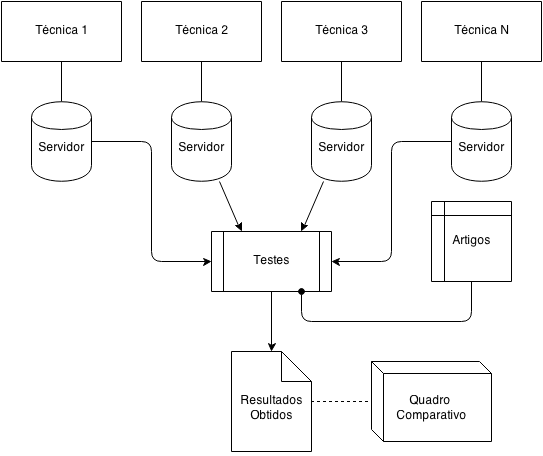
\includegraphics[width=0.7\linewidth]{./assets/metodology}
\end{figure}


\section{Seleção das Técnicas/Ferramentas}

As técnicas que foram analisadas dentro do capítulo de \textbf{Revisão de Literatura} compreendem um universo atuante e de caráter livre, independente da linguagem de programação que foi utilizada no desenvolvimento, exceto pelos detalhes explicados nas limitações do trabalho.

Em função do grande número de ferramentas disponíveis como resultado desta pesquisa, algumas foram selecionadas a fim de se obter ao máximo os testes e os resultados esperados.

Conforme mencionado anteriormente, ferramentas pagas ou que não disponibilizam o código para instalação não foram testadas, visto que a necessidade do atual trabalho visa identificar os resultados obtidos dentro de um conjunto de infra estrutura única, de maneira justa com cada projeto.

Assim sendo, a tabela \ref{tab:ferramentas} lista as seguintes ferramentas que foram selecionadas para teste dentro do escopo proposto neste trabalho.

% Colocar uma tabela com as técnicas que serão comparadas

\begin{table}
    \caption{Ferramentas selecionadas para testes}
    \begin{center}
    	\begin{tabular}{|p{6cm}|p{5cm}|}
			\hline \textbf{Ferramenta} & \textbf{Linguagem} \\ 
			\hline Ferramenta 1 & Java\\
			\hline Ferramenta 2 & Perl\\
			\hline Ferramenta 3 & Python\\
			\hline Ferramenta 4 & Java\\
	    	\hline 
    	\end{tabular} 
    \end{center}
  	\label{tab:ferramentas}
\end{table}

\section{Seleção de Artigos}

Visando provar a eficiência destas técnicas, desejamos ter informações de saída consideradas corretas para que seus resultados possam ser comparados e verificados com exatidão. Assim, foi selecionada uma série de artigos científicos das mais diversas áreas de pesquisa, de diversos eventos distintos, com padrões visuais totalmente diferentes e que são possível de ser analisados e coletados.

% Áreas dos Artigos e Eventos

Desde modo a lista destes artigos compreende um total de 100 documentos variados, com seus metadados já extraídos manualmente e todos catalogados a fim de ter o resultado da aplicação das técnicas comparado com os resultados obtidos manualmente. Na Tabela \ref{tab:papers-list} pode-se ver o número de artigos que foram selecionados por cada área do conhecimento. A relação de todos os artigos analisados pode ser obtida no Anexo \ref{anexo-artigos} deste documento.

Os artigos foram selecionados tomando como base a principal forma de análise das técnicas selecionadas para testes: o layout, ou seja, a disposição dos elementos nos artigos científicos. Esta seleção foi feite com base a abranger um maior número de representações, com disposições diferentes, tipografias diferentes e inclusive ordem diferentes nas exibições. Desta forma as técnicas poderão ser confrontadas e os resultados comparados com os resultados esperados.

% Artigos em Inglês, somente

Todos os artigos selecionados foram escritos na língua inglesa. Esta decisão foi tomada em virtude de além de ser a língua inglesa universal para disseminação de conhecimento, ela é a mais utilizada no meio acadêmico, de maneira a ter um universo muito maior de artigos escrito em inglês do que outras línguas.

Além disso a abrangência de outros idiomas entraria em um aspecto que não é objetivo deste trabalho abordar, visto a diversificação de culturas e símbolos, fazendo com que línguas orientais, como o mandarim ou japonês, tenham análises diferenciadas em função de suas diferenças na forma de representação.

\begin{table}
    \caption{Seleção de artigos científicos para testes (ainda em desenvolvimento)}
    \begin{center}
        \begin{tabular}{|l|l|}
        	\hline
            \textbf{Área de Conhecimento} & \textbf{Total de Artigos} \\ 
            \hline
            Arquitetura e Urbanismo & 7 \\ 
			Música & 7 \\ 
			Ciência da Computação & 8 \\
			Ciência da Informação & 9 \\
            Ciências Biológicas & 7 \\
            Direito & 7 \\
            Engenharia Civil & 8 \\
            Letras & 7 \\
            Matemática Computacional & 7 \\
            Medicina & 9 \\ 
            Odontologia & 8 \\ 
            Psicologia & 9 \\
            Sociologia & 7 \\	
            \hline
            \textbf{Total} & \textbf{100} \\
            \hline 
        \end{tabular}
    \end{center}
    \label{tab:papers-list}
\end{table}

\section{Infraestrutura Computacional}

Para que os testes sejam feitos de maneira adequada e independente, sem interferência de outras técnicas nos resultados, serão utilizados N servidores, sendo N o número total de técnicas a serem avaliadas.

Deste modo, para cada técnica avaliada será configurado um servidor com as linguagens de programação necessárias e todos os pré-requisitos que a técnica necessita para funcionar. Estes servidores serão definidos através de máquinas virtuais, o que traz benefícios não somente de performance mas de flexibilidade quanto das tecnologias necessárias para o funcionamento de cada técnica.

\subsection{Testes In Loco}

% Falar de técnicas que já possuem algum site para testes, demonstrando a ferramente funcionando

Algumas técnicas de extração de metadados disponibilizam acesso online a uma ferramenta gratuita para testes. Deste modo, para estes casos específicos não será necessária a criação de servidores e instalação dos pacotes, visto que o ambiente de testes poderá ser feito dentro da ferramente fornecida pelas desenvolvedoras das técnicas.

% Vantagem de ser feito o teste online

Este fato garante uma maior precisão nos resultados, inclusive pelo fato de o ambiente de testes estar 100\% funcionando e ter sido disponibilizado pela mesma equipe de desenvolvedores do projeto, garantindo a eficácia nos resultados que essa técnicas fornece.

\section{Quadro Comparativo}

Visando uma comparação dos resultados eficaz todos os resultados serão inseridos em um documento formato planilha para serem comparados manualmente e as conclusões então obtidas. Para tal esta planilha de resultados a chamaremos de "Quadro Comparativo" e será exclusiva para comparação dos resultados das técnicas analisadas.

% Formato online para consulta futura

Com o objetivo de facilitar o acesso às informações este documento é disponibilizado como anexo deste projeto e ainda tem seu acesso liberado em formato online. Desta forma qualquer pessoa poderá ter acesso aos resultados obtidos pelos testes e comparar elas mesmas os dados contidos na planilha.

\section{Metadados, Pesos e Resultados}

% Importância de se ter pesos em função dos metadados

A extração de metadados de artigos científicos engloba um processo onde os resultados obtidos, mais especificamente os metadados propriamente ditos, possuem características diferenciadas que podem influenciar em uma busca por artigos, feita por um pesquisador.

Desde modo atribuímos pesos para cada um dos metadados analisados, de maneira a identificar os mais importantes e que podem contribuir com um número maior de resultados de busca. 

% Quais metadados são mais importantes para uma pesquisa de artigos

Alguns metadados são mais importantes que outros no que diz respeito à funcionalidade de pesquisa. Geralmente quando vamos buscar artigos, seja na Internet, ou em algum outro local, geralmente buscamos primeiro pelo título do artigo (quando procuramos por um artigo em específico) ou então pelo nome do autor (quanto procuramos artigos de um determinado autor).

Além disso, utilizamos também o título, juntamente com o resumo, para buscar de palavras chaves ou palavras que podem ser relevantes na pesquisa pelos documentos. Assim sendo alguns metadados devem ser mais considerados no resultado destas extrações, por serem mais importantes no ponto de vista da busca.

Assim sendo apresentamos a tabela \ref{tab:pesos}, que demonstra como cada metadado teve sua importância interpretada e qual o peso que lhe foi atribuído, sendo utilizado o inteiro 1 para o peso mais baixo e o 5 para peso mais alto, sendo consequentemente o mais importantes.

% Tabela de metadados e pesos

\begin{table}
    \caption{Os metadados e seus pesos atribuídos}
    \begin{center}
    	\begin{tabular}{|p{3cm}|p{8cm}|C{1cm}|}
			\hline \textbf{Metadado} & \textbf{Relevância} & \textbf{Peso} \\ 
			\hline Título & Um dos termos mais buscados quando se pesquisa um artigo & 5 \\
	    	\hline Autor(es) & O segundo termo mais pesquisado & 4 \\
	    	\hline E-mail(s) & Pouco relevante no quesito pesquisa de artigos & 1 \\
	    	\hline Resumo & Importante por conter palavras chaves e o resumo propriamente dito & 3 \\
	    	\hline Referências & Muito importante e necessário, pois será utilizada na referência inversa de autores & 5 \\
	    	\hline 
    	\end{tabular} 
    \end{center}
  	\label{tab:pesos}
\end{table}

% Falar sobre a porcentagem de acertos em cada metadado, por exemplo, se o resultado extraiu 90\% do resultado (não a totalidade), deve ser considerado um valor para este resultado, não somente sim ou não.

Outro detalhe importante é a precisão de cada resultado para cada metadado analisado. Em alguns casos o título, por exemplo, não é extraído em 100\% mas alguma variação dele. 

Deste modo consideramos 3 (três) resultados possíveis para um resultado analisado:

\begin{enumerate}
\item \textbf{Preciso:} Quando um resultado atinge acima de 95\% de precisão, ou seja, o campo foi extraído em 95\% ou mais de sua totalidade.
\item \textbf{Satisfatório:} Quando um resultado atinge entre 90 e 94\%, o que pode ser considerado satisfatório e a maioria do conteúdo consegue ser analisada sem maiores problemas.
\item \textbf{Inaceitável:} Quando o resultado atinge abaixo de 90\%, ou seja, entre 0\% e 89\%. Este resultado no âmbito do presente projeto é considerado inaceitável.
\end{enumerate}

Assim, temos o valor de cada resultado possível, que será também utilizado no processo de análise, conforme consta na tabela \ref{tab:precisao}. Cada valor, independente de sua classificação será utilizado para o cálculo final da nota de cada ferramenta.

% Tabela de precisão e os valores

\begin{table}
    \caption{Resultados obtidos em cada metadado e sua precisão}
    \begin{center}
    	\begin{tabular}{|C{3cm}|C{3cm}|}
			\hline \textbf{Resultado} & \textbf{Precisão} \\ 
			\hline Preciso & 1\\
	    	\hline Satisfatório & 0.60 \\
	    	\hline Inaceitável & 0 \\
	    	\hline 
    	\end{tabular} 
    \end{center}
  	\label{tab:precisao}
\end{table}

\subsection{Índice de Confiabilidade}

% Fórmula final para a nota final de cada técnica

Considerando que cada metadado possui um peso diferente necessitamos calcular o índice de acertos a ser utilizado em cada resultado coletado para cada técnica aplicada. Assim sendo chegamos em uma fórmula matemática à qual chamamos "Índice de Confiabilidade", que calcula o resultado obtido através dos pesos que foram atribuídos a cada campo.

Este índice utiliza os pesos anteriormente definidos e a precisão dos resultados obtida, de maneira a permitir chegar em uma única nota final para cada técnica aplicada.

Basicamente a fórmula atua como uma média ponderada dos resultados alcançados na extração de cada campo do artigo, seguindo os pesos apresentados em \ref{tab:pesos}. Cada peso é atribuído ao resultado encontrado em cada ferramenta testada. 

A título de exemplo, após o teste de uma ferramenta, supondo que ela conseguiu extrair 87\% dos títulos dos artigos com sucesso, sua precisão com relação ao título será 87, que será multiplicado pelo peso correspondendo ao seu campo, neste caso, o inteiro 5. Isso ocorre para todos os campos apresentados, seguindo seus respectivos pesos.

A descrição de cada variável no Índice de Confiabilidade poderá ser obtida de acordo com a tabela \ref{tab:indice-confidencialidade}, onde temos as variáveis que fazem parte da fórmula descrita.

\begin{center}
	$ IC=\frac{5(PT)+4(PA)+PE+3(PR)+5(PRF)}{18} $
\end{center}

\begin{table}
    \caption{Descrição de cada variável no Índice de Confiabilidade}
    \begin{center}
    	\begin{tabular}{|p{3cm}|p{8cm}|}
			\hline \textbf{Variável} & \textbf{Descrição}\\ 
			\hline PT & Precisão na obtenção do título \\
			\hline PA & Precisão na obtenção do(s) autor(es)\\
			\hline PE & Precisão na obtenção dos e-mails dos autores \\
			\hline PR & Precisão na obtenção do resumo \\
			\hline PRF & Precisão na obtenção das referências \\
	    	\hline 
    	\end{tabular} 
    \end{center}
  	\label{tab:indice-confidencialidade}
\end{table}

% Análise e Apresentação de Resultados
\chapter{Análise e Apresentação de Resultados}

% Construção da teoria

Com base no objetivo de identificar como as ferramentas atuais se comportam nos mais diversos tipos de padrões visuais foram realizados vários experimentos práticos a fim de obter os resultados numéricos desejados para que o objetivo fosse alcançado.

Desta maneira, foram separadas algumas ferramentas/técnicas implementáveis tecnicamente para que os artigos selecionados (citados no capítulo anterior) pudessem ser analisados e seus dados extraídos segundo os propósitos de cada uma.

% Conceitos criados pelo autor

Para que os resultados pudessem ser medidos e comparados foi utilizado o "Índice de Confiabilidade" detalhado no capítulo de \textbf{Metodologia}, a fim de obter um valor numérico para cada resultado apresentado com a utilização das ferramentas, permitindo que os valores obtidos fossem comparados e então confrontados para se obter o comportamento de cada ferramenta.

% Trabalhar as evidências de que sua hipótese é verdadeira

% Apresentar dados, testes, provas, estudos de caso, etc

\section{Ambiente de Testes}

Para que esta análise pudesse ser feita com exatidão e garantir assim os resultados esperados, foi-se criado um ambiente de testes abrangendo um conjunto de tecnologias para que as ferramentas pudessem ser instaladas e testas seguindo o propósito de cada uma.

\subsection{Servidores de Teste}

Para cada teste de ferramenta foi criada uma Máquina Virtual dentro do Ambiente de Testes, com o objetivo de ter plataformas operando independentemente, com apenas as tecnologias necessárias para seu correto funcionamento, sem influência de códigos terceiro e/ou programas desnecessários.

Por restringir apenas os testes utilizando ferramentas de código livre, todos os testes realizados ocorreram em máquinas Linux\footnote{Sistema operacional de código livre com ampla utilização em servidores de todo o mundo.}, de acordo com a Tabela \ref{tab:lista-servidores}, respeitando os requisitos necessários para cada ferramenta.

\begin{table}
    \caption{Ferramentas e Ambientes de Testes}
    \begin{center}
    	\begin{tabular}{|p{3cm}|p{8cm}|}
			\hline \textbf{Ferramenta} & \textbf{Ambiente}\\ 
			\hline Ferramenta 1 & Linux Ubuntu 12.04, Java 7, Sqlite, Tomcat 6 \\
			\hline Ferramenta 2 & Linux Ubuntu 12.04, Perl, MySQL, Nginx \\
			\hline Ferramenta 3 & Linux Ubuntu 12.04, Perl, PostgreSQL, Apache \\
			\hline Ferramenta 4 & Linux Ubuntu 12.04, Java 6, MySQL, Tomcat 6 \\
	    	\hline 
    	\end{tabular} 
    \end{center}
  	\label{tab:lista-servidores}
\end{table}

% Conclusao
\chapter{Discussão / Trabalhos Futuros}

% Analisar os objetivos gerais e específicos e explicar como o desenvolvimento ajudou a chegar em cada um destes objetivos
% Apresentar os pontos positivos e negativos do trabalho também
% Lições aprendidas

% "... o problema descrico na seção X foi resolvido como demonstrado nas sessões y a z, em que foi desenvolvido um algoritmo/método/abordagem etc para tratar as situações mencionadas.



\section{Contribuições}


\section{Trabalhos Futuros}

% Futuras contribuições ao conhecimento com mais ênfase do que futuras contribuições às ferramentas, protótipos, etc, que eventualmente possa, ser desenvolvidas

% Falar sobre oportunidades de pesquisa nesta área, que o autor não conseguiu averiguar, mas serve de dicas para os próximos interessados

% Exemplo, falar quais situações ainda não foram feitos os testes, que podem ser feitos no futuro para compreender alguma coisa por exemplo



% 

\section{Considerações Finais}



% ---

% ----------------------------------------------------------
% ELEMENTOS PÓS-TEXTUAIS
% ----------------------------------------------------------
\postextual
% ----------------------------------------------------------

% ----------------------------------------------------------
% Referências bibliográficas
% ----------------------------------------------------------
\bibliography{includes/referencias}

% ----------------------------------------------------------
% Glossário
% ----------------------------------------------------------
%
% Consulte o manual da classe abntex2 para orientações sobre o glossário.
%
%\glossary

% ----------------------------------------------------------
% Apêndices
% ----------------------------------------------------------

% ---
% Inicia os apêndices
% ---
% \begin{apendicesenv}

% % Imprime uma página indicando o início dos apêndices
% \partapendices

% % ----------------------------------------------------------
% \chapter{Quisque libero justo}
% % ----------------------------------------------------------

% \lipsum[50]

% % ----------------------------------------------------------
% \chapter{Nullam elementum urna vel imperdiet sodales elit ipsum pharetra ligula
% ac pretium ante justo a nulla curabitur tristique arcu eu metus}
% % ----------------------------------------------------------
% \lipsum[55-57]

% \end{apendicesenv}
% ---


% ----------------------------------------------------------
% Anexos
% ----------------------------------------------------------

% ---
% Inicia os anexos
% ---
\begin{anexosenv}

% Imprime uma página indicando o início dos anexos
\partanexos

% ---
\chapter{Elementos do padrão Dublin Core, versão 1.1}
\label{anexo-dublin-core}
% ---

\begin{flushleft}

    \begin{longtable}{|p{2cm}|p{2cm}|p{4cm}|p{6cm}|}
        \hline \textbf{Name} & \textbf{Label} & \textbf{Definition} & \textbf{Comment}\\ 
        \hline title & Title & A name given to the resource. & \\
		\hline creator & Creator & An entity primarily responsible for making the resource. & Examples of a Creator include a person, an organization, or a service.  Typically, the name of a Creator should be used to indicate the entity.\\
		\hline subject & Subject & The topic of the resource. & Typically, the subject will be represented using keywords, key phrases, or classification codes. Recommended best practice is to use a controlled vocabulary. To describe the spatial or temporal topic of the resource, use the Coverage element.\\
		\hline description & Description & An account of the resource. & Description may include but is not limited to: an abstract, a table of contents, a graphical representation, or a free-text account of the resource.\\
        \hline publisher & Publisher & An entity responsible for making the resource available. & Examples of a Publisher include a person, an organization, or a service.  Typically, the name of a Publisher should be used to indicate the entity.\\
		\hline contributor & Contributor & An entity responsible for making contributions to the resource. & Examples of a Contributor include a person, an organization, or a service. Typically, the name of a Contributor should be used to indicate the entity.\\
        \hline date & Date & A point or period of time associated with an event in the lifecycle of the resource. & Date may be used to express temporal information at any level of granularity.  Recommended best practice is to use an encoding scheme, such as the W3CDTF profile of ISO 8601 [W3CDTF].\\
        \hline type & Type & The nature or genre of the resource. & Recommended best practice is to use a controlled vocabulary such as the DCMI Type Vocabulary [DCTYPE]. To describe the file format, physical medium, or dimensions of the resource, use the Format element.\\
        \hline format & Format & The file format, physical medium, or dimensions of the resource. & Examples of dimensions include size and duration. Recommended best practice is to use a controlled vocabulary such as the list of Internet Media Types [MIME].\\
        \hline identifier & Identifier & An unambiguous reference to the resource within a given context. & Recommended best practice is to identify the resource by means of a string conforming to a formal identification system.\\
        \hline source & Source & A related resource from which the described resource is derived. & The described resource may be derived from the related resource in whole or in part.  Recommended best practice is to identify the related resource by means of a string conforming to a formal identification system.\\
        \hline language & Language & A language of the resource. & Recommended best practice is to use a controlled vocabulary such as RFC 4646 [RFC4646].\\
        \hline relation & Relation & A related resource. & Recommended best practice is to identify the related resource by means of a string conforming to a formal identification system.\\
        \hline coverage & Coverage & The spatial or temporal topic of the resource, the spatial applicability of the resource, or the jurisdiction under which the resource is relevant. & Spatial topic and spatial applicability may be a named place or a location specified by its geographic coordinates.  Temporal topic may be a named period, date, or date range.  A jurisdiction may be a named administrative entity or a geographic place to which the resource applies.  Recommended best practice is to use a controlled vocabulary such as the Thesaurus of Geographic Names [TGN].  Where appropriate, named places or time periods can be used in preference to numeric identifiers such as sets of coordinates or date ranges.\\
        \hline rights & Rights & Information about rights held in and over the resource. & Typically, rights information includes a statement about various property rights associated with the resource, including intellectual property rights.\\
        \hline
    \end{longtable}

\end{flushleft}

% ---
\chapter{Listagem de artigos analisados para realização do experimento}
\label{anexo-artigos}
% ---

\begin{flushleft}
	\begin{longtable}{|C{0.6cm}|m{10.1cm}|C{4cm}|}
		\hline
	    \# & \textbf{Título \textit{(Autores)}} & \textbf{Área/Disciplina} \\ 
	    \hline
	    \rownumber & Benefits of extra-pair mating may depend on environmental conditions—an experimental study in the blue tit
(Cyanistes caeruleus) \textit{(Aneta Arct, Szymon M. Drobniak, Edyta Podmokta, Lars Gustafson, Mariusz Cichoń)} & Ciências Biológicas \\
		\hline
		\rownumber & Cost-Effective Suppression and Eradication of Invasive Predators \textit{(Peter W. J. Baxter, John L. Sabo, Chris Wilcox, Michael A. McCarthy, Hugh P. Possingham)} & Ciências Biológicas \\
		\hline
		\rownumber & Model selection and model averaging in behavioural ecology: the utility of the IT-AIC framework \textit{(Shane A. Richards, Mark J. Whittingham, Philip A. Stephens)} & Ciências Biológicas \\
		\hline
		\rownumber & Territory size of the flavescent warbler, Basileuterus flaveolus (Passeriformes, Emberizidae), in a forest fragment in Southeastern Brazil \textit{(Charles Duca, Miguel Â. Marini)} & Ciências Biológicas \\
		\hline
		\rownumber & Effectiveness of Corridors Relative to Enlargement of Habitat Patches \textit{(Mattew R. Falcy, Cristián F. Estades)} & Ciências Biológicas \\
		\hline
		\rownumber & High fidelity on islands: a comparative study of extrapair paternity in passerine birds \textit{(Simon C. Griffith)} & Ciências Biológicas \\
		\hline
		\rownumber & Parentage and Relatedness in Polyandrous Comb-Crested Jacanas Using ISSRs \textit{(S. M. Haig, T. R. Mace, T. D. Mullins)} & Ciências Biológicas \\
		\hline
		\rownumber & Factors influencing double brooding in Eurasian Hoopoes Upupa epops \textit{(Jael Hoffmann, Erik Postma, Michael Schaub)} & Ciências Biológicas \\
		\hline
		\rownumber & The importance of fission–fusion social group dynamics in birds \textit{(Matthew J. Silk, Darren P. Croft, Tom Tregenza, Stuart Bearhop)} & Ciências Biológicas \\
		\hline
		\rownumber & Genetic monogamy in two long-lived New Zealand passerines \textit{(Sabrina S. Taylor, Sanne Boessenkool, Ian G. Jamieson)} & Ciências Biológicas \\
	    \hline
	    \rownumber & A Probabilistic Framework for Semi-Supervised Clustering \textit{(Sugato Basu, Mikhail Bilenko, Raymond J. Mooney)} & Ciência da Computação\\
	    \hline
	    \rownumber & Document Clustering: The Next Frontier \textit{(David C. Anastasiu, Andrea Tagarelli, George Karypis)} & Ciência da Computação\\
	    \hline
	    \rownumber & Enhancing Semi-Supervised Document Clustering with Feature Supervision \textit{(Yeming Hu, Evangelos E. Milios, James Blustein)} & Ciência da Computação\\
	    \hline
	    \rownumber & Instance-Level Constraint-Based Semisupervised Learning With Imposed Space-Partitioning \textit{(Jayaram Raghuram, David J. Miller, George Kesidis)} & Ciência da Computação\\
		\hline
		\rownumber & Alternatives to the k-means algorithm that find better clusterings \textit{(Greg Hamerly, Charles Elkan)} & Ciência da Computação\\
		\hline
		\rownumber & Towards Parameter-Free Data Mining \textit{(Eamonn Keogh, Stefano Lonardi, Chotirat Ann Ratanamahatana)} & Ciência da Computação\\
		\hline
		\rownumber & Learning Nonparametric Kernel Matrices from Pairwise Constraints \textit{(Steven C. H. Hoi, Rong Jin, Michael R. Lyu)} & Ciência da Computação\\
		\hline
		\rownumber & Enhancing Semi-Supervised Clustering: A Feature Projection Perspective \textit{(Wei Tang, Hui Xiong, Shi Zhong, Jie Wu)} & Ciência da Computação\\
		\hline
		\rownumber & Integrating Constraints and Metric Learning in Semi-Supervised Clustering \textit{(Mikhail Bilenko, Sugato Basu, Raymond J. Mooney)} & Ciência da Computação\\
		\hline
		\rownumber & On Weighting Clustering \textit{(Richard Nock, Frank Nielsen)} & Ciência da Computação\\
	    \hline
	    \rownumber & Masculinity, Sexuality and the Body of Male Soldiers \textit{(Nyameka Mankayi)} & Psicologia \\
	    \hline
	    \rownumber & Consumption of alcohol and depression in students of a public school of CoatzaCoalCos, VeraCruz, Mexico \textit{(Brenda Alicia Hernández-Cortaza, Leticia Cortaza-Ramirez, Moacyr Lobo da Costa Junior)} & Psicologia \\
	    \hline
	    \rownumber & Psychometric Properties of the Spanish Language Version of the Stress in Children Questionnaire (SiC) \textit{(Alejandra Caqueo-Urízar, Alfonso Urzúa, Walter Osika)} & Psicologia \\
	    \hline
	    \rownumber & Facial information processing in schizophrenia \textit{(João Paulo Machado de Sousa, Jaime Eduardo Cecílio Hallak)} & Psicologia \\
	    \hline
	    \rownumber & Intelligence and socioeconomic success: A meta-analytic review of longitudinal research \textit{(Tarmo Strenze)} & Psicologia \\
	    \hline
	    \rownumber & The Science of Sex Differences in Science and Mathematics \textit{(Diane F. Halpern, Camilla P. Benbow, David C. Geary, Ruben C. Gur, Janet Shibley Hyde, Morton Ann Gernsbacher)} & Psicologia \\
	    \hline
	    \rownumber & Hardiness and Burnout Syndrome: A Cross-Cultural Study among Portuguese and Brazilian Nurses \textit{(Mary Sandra Carlotto, Cristina Queirós, Sofia Dias, Mariana Kaiseler)} & Psicologia \\
	    \hline
	    \rownumber & Social Psychology: Fundamentals and Fundamentalisms \textit{(Marcus Eugênio Oliveira Lima)} & Psicologia \\
	    \hline
	    \rownumber & Computerized Assessment of Food Preferences in Adolescents in the Stimulus Equivalence Paradigm \textit{(Gisele Straatmann, Sebastião Sousa Almeida, Julio C. de Rose)} & Psicologia \\
	    
	    \hline
	\end{longtable}
\end{flushleft}

%\begin{table}
%	\caption{Teste}
%    \begin{center}
%        
%    \end{center}
%    \label{tab:papers-list-total}
%\end{table}

\end{anexosenv}



%---------------------------------------------------------------------
% INDICE REMISSIVO
%---------------------------------------------------------------------
\phantompart
\printindex
%---------------------------------------------------------------------

\end{document}
